
\section*{Use cases}

\begin{frame}{Use cases}
  \begin{columns}[c]
    
    \begin{column}{.5\textwidth}
      \begin{figure}
        \centering
        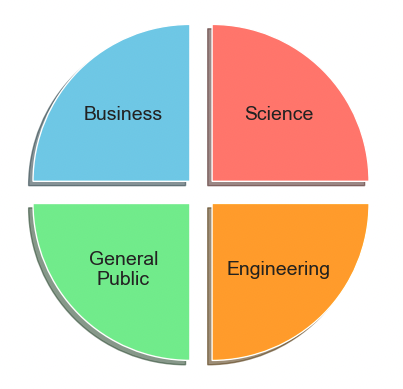
\includegraphics[width=\textwidth]{img/viz/pie-level-tech.png}
      \end{figure}
    \end{column}
    
    \begin{column}{.5\textwidth}
      \begin{itemize}
        \item Wide range of use cases
        \item Various fields
        \item Differents levels of understanding of the data visualization concepts
      \end{itemize}
    \end{column}

  \end{columns}
\end{frame}


\begin{frame}{Use cases / General public}
  \textbf{Public health}

  \centering
  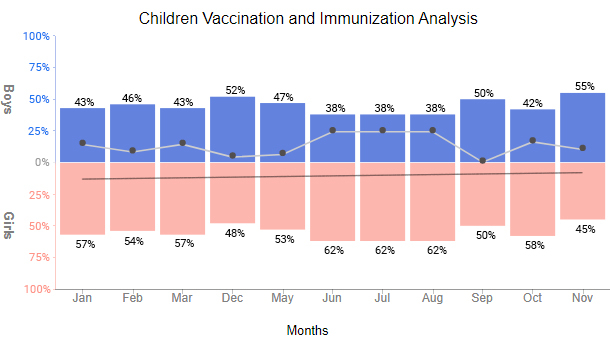
\includegraphics[width=\textwidth]{img/viz/uc-healthcare.jpg}

% ref: https://chartexpo.com/blog/healthcare-data-visualization#
\end{frame}


\begin{frame}{Use cases / General public}
  \textbf{Statistics about populations}

  \centering
  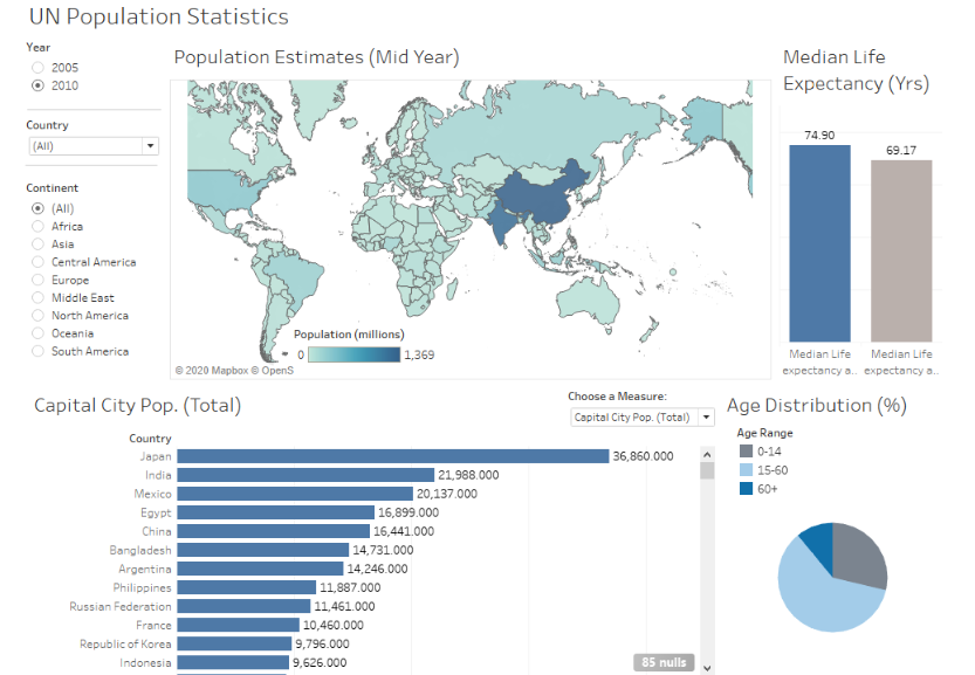
\includegraphics[width=\textwidth]{img/viz/uc-population.png}

  % Ref: https://www.linkedin.com/pulse/visualizing-un-population-data-ruth-cheng/
\end{frame}

\begin{frame}{Use cases / General public}
  \textbf{Environmental and climate change}

  \centering
  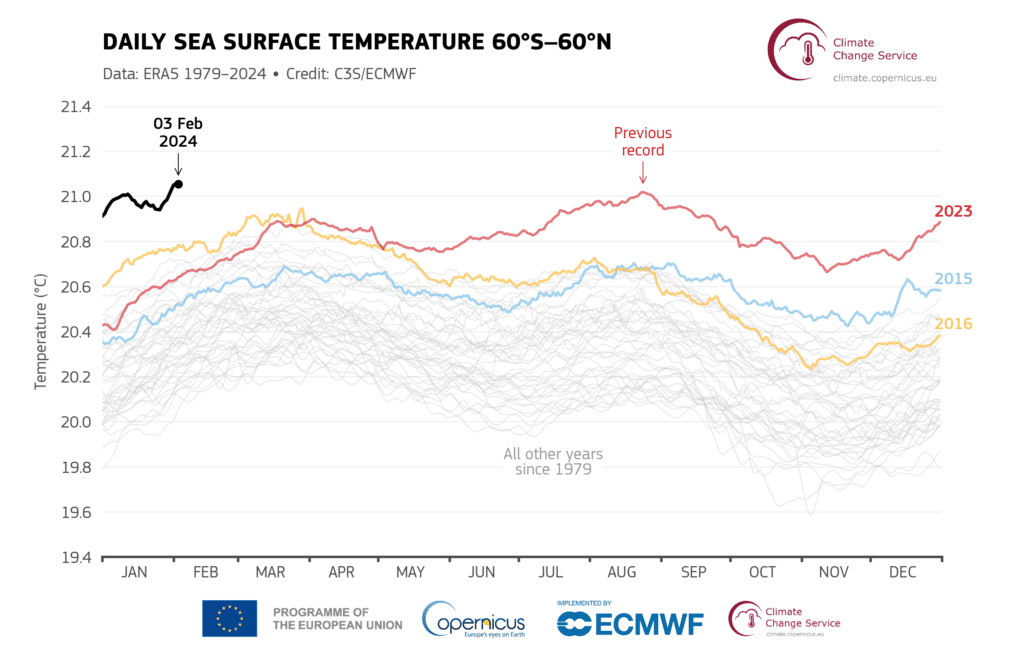
\includegraphics[width=\textwidth]{img/viz/uc-climate.png}
\end{frame}



\begin{frame}{Use cases / Business}
  \textbf{Business Intelligence (BI) and Analytics}

  \centering
  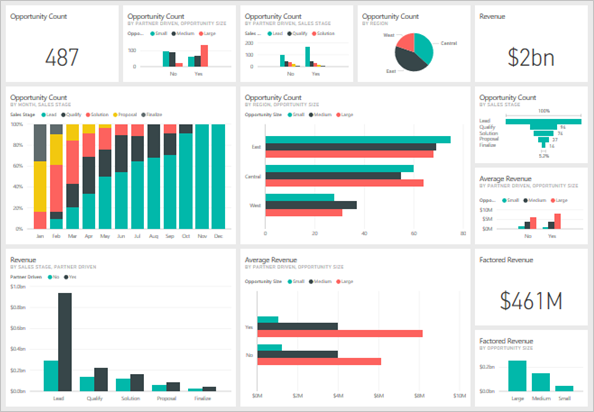
\includegraphics[width=\textwidth]{img/viz/Power_BI_dashboard.png}
\end{frame}

\begin{frame}{Use cases / Business}
  \textbf{Finance}

  \centering
  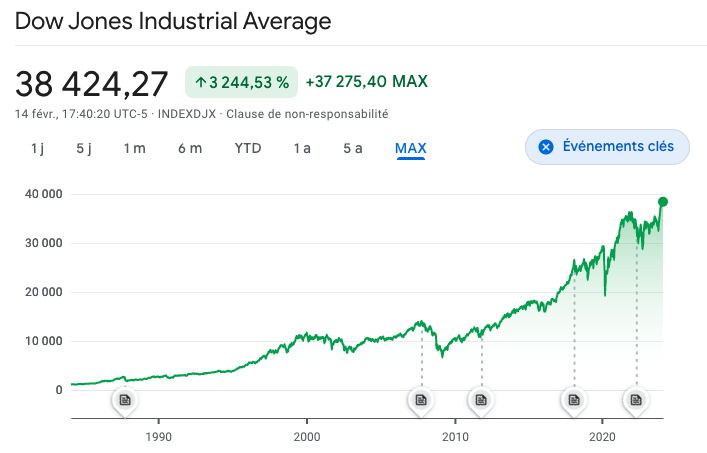
\includegraphics[width=\textwidth]{img/viz/uc-finance.png}
\end{frame}

\begin{frame}{Use cases / Business}
  \textbf{Project management}

  \centering
  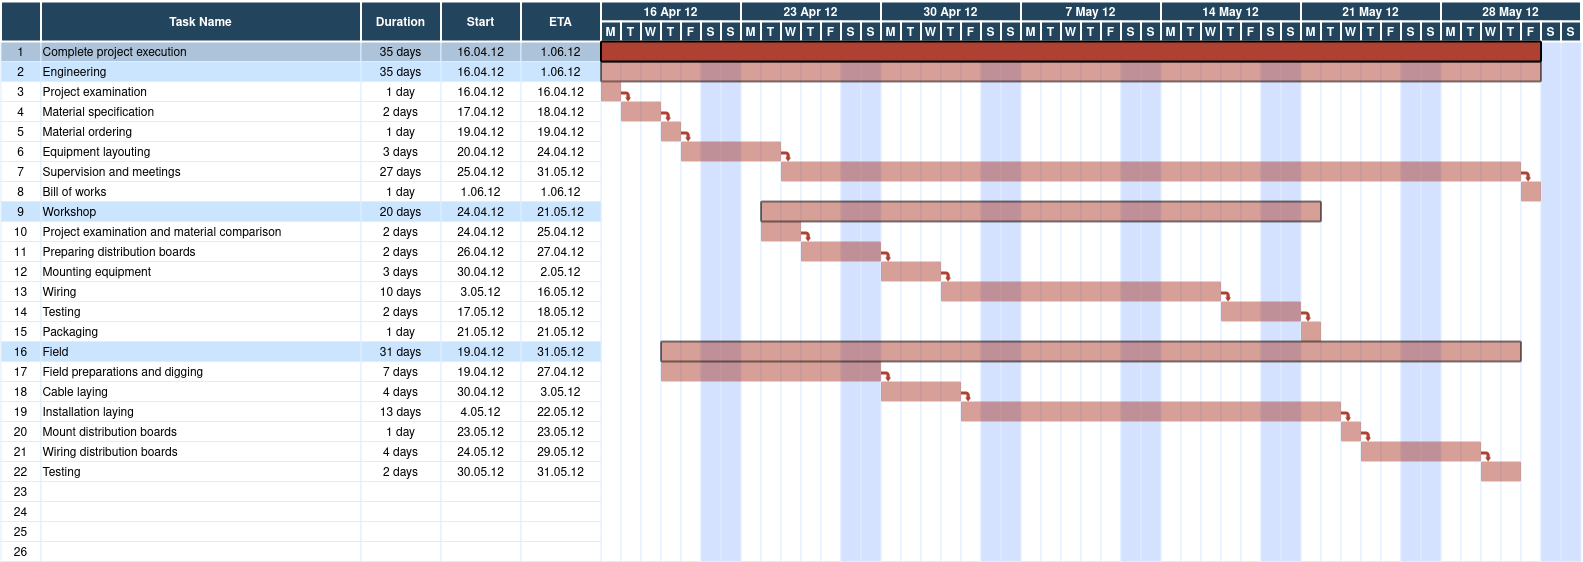
\includegraphics[width=\textwidth]{img/viz/gantt.png}
\end{frame}

\begin{frame}{Use cases / Business}
  \textbf{Team management}

  \centering
  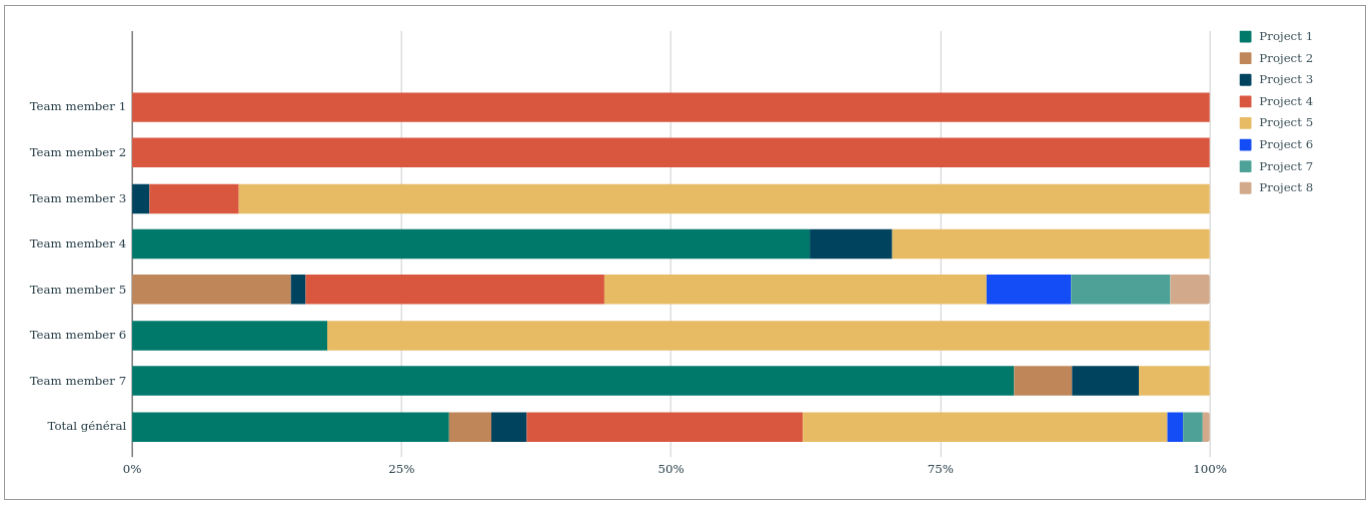
\includegraphics[width=\textwidth]{img/viz/time_tracking.png}
\end{frame}


\begin{frame}{Use cases / Engineering}
  \textbf{Anomaly detection}

  \centering
  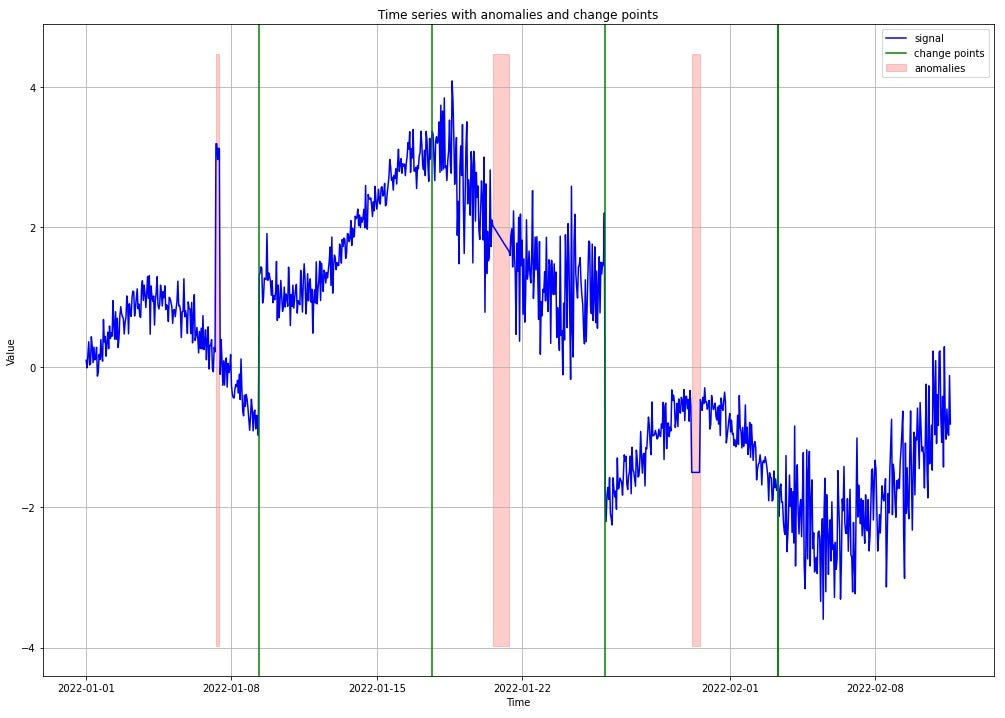
\includegraphics[width=\textwidth]{img/viz/uc-anomaly.jpg}

\end{frame}


\begin{frame}{Use cases / Engineering}
  \textbf{Urban Planning and Transportation}

  \centering
  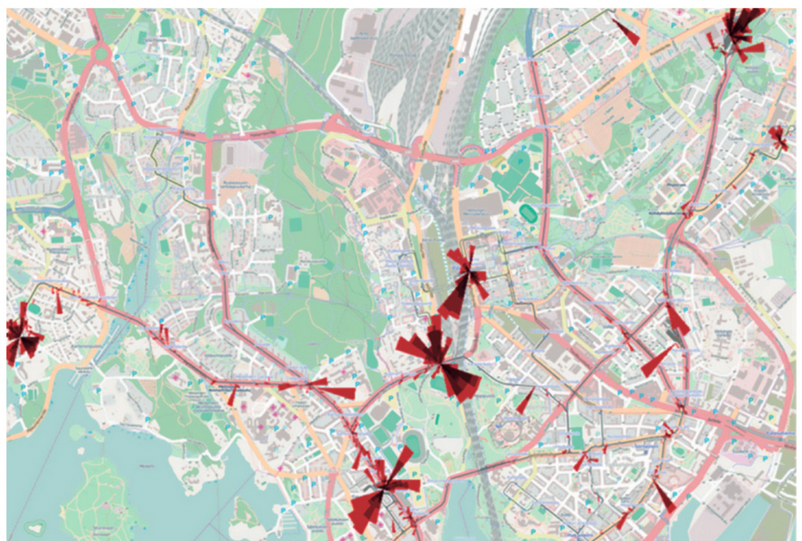
\includegraphics[width=\textwidth]{img/viz/uc-transport.png}
  % ref: https://www.mdpi.com/1424-8220/19/2/332
\end{frame}
 
\begin{frame}{Use cases / Science}
  \textbf{Data science and Machine learning}

  \centering
  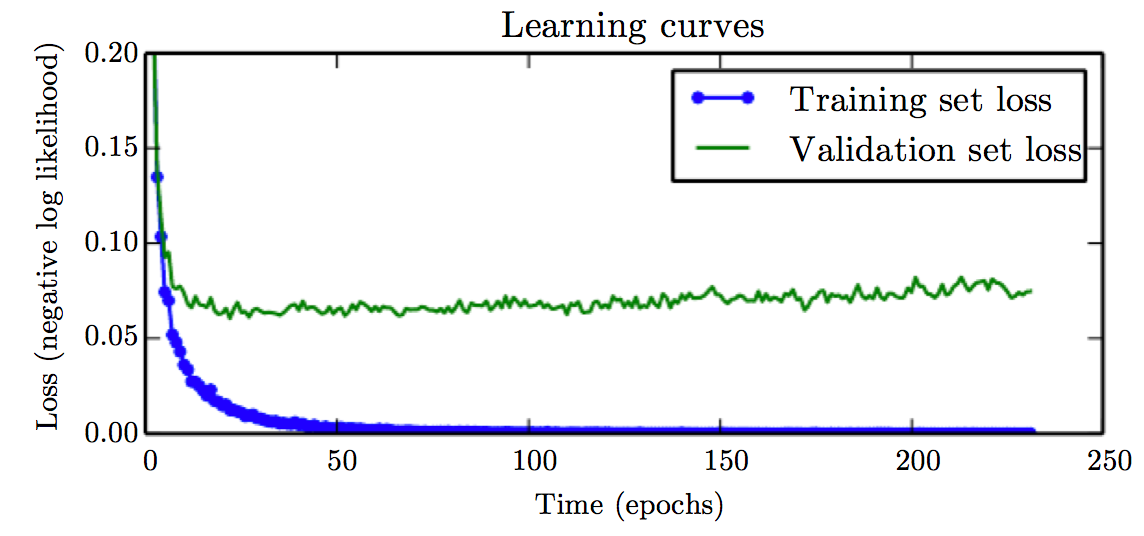
\includegraphics[width=\textwidth]{img/viz/early-stopping.png}
\end{frame}

\begin{frame}{Use cases / Science}
  \textbf{Data analysis}

  \centering
  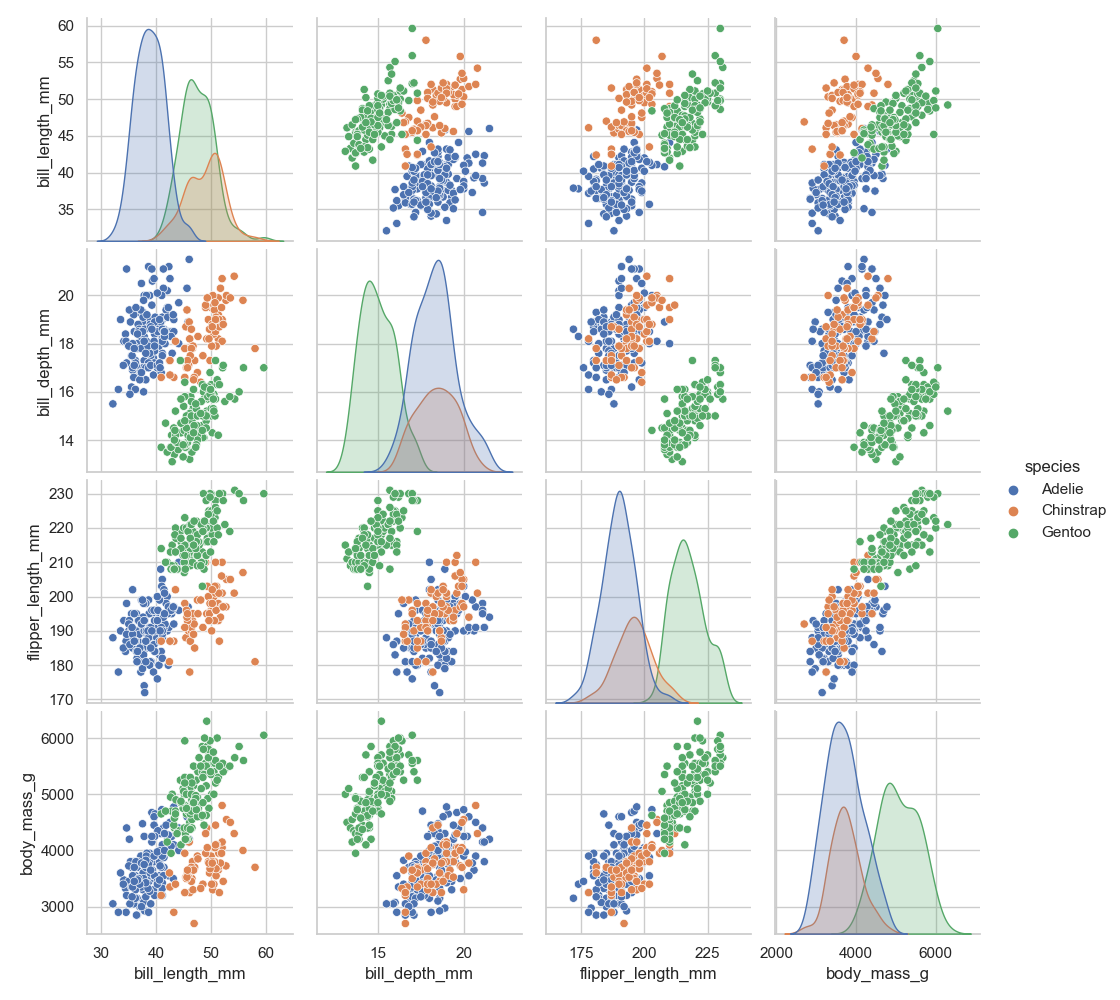
\includegraphics[width=0.8\textwidth]{img/viz/scatterplot_matrix_2.png}
\end{frame}

\begin{frame}{Use cases / Science}
  \textbf{Big data analysis}

  \centering
  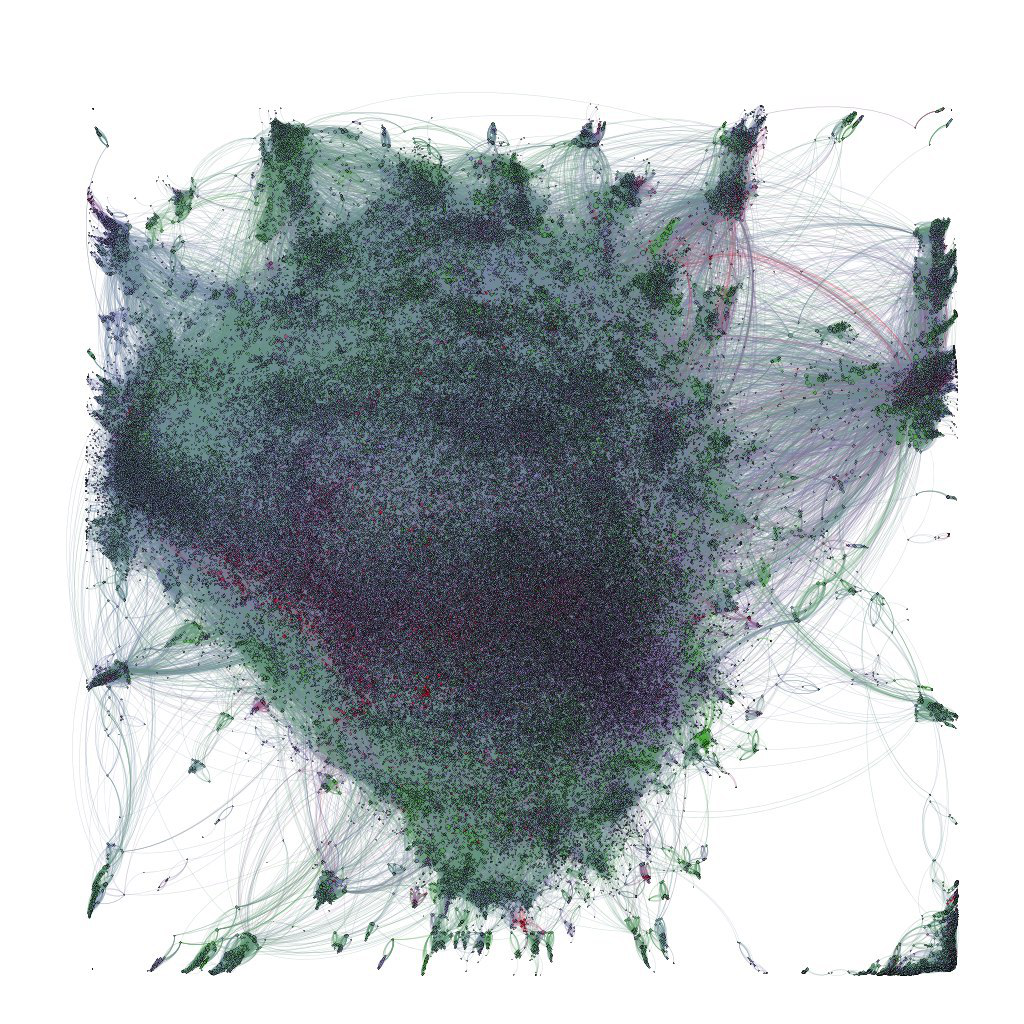
\includegraphics[width=0.8\textwidth]{img/viz/large_graph.png}
\end{frame}


\section*{Softwares}

\begin{frame}{Softwares}
  \centering
  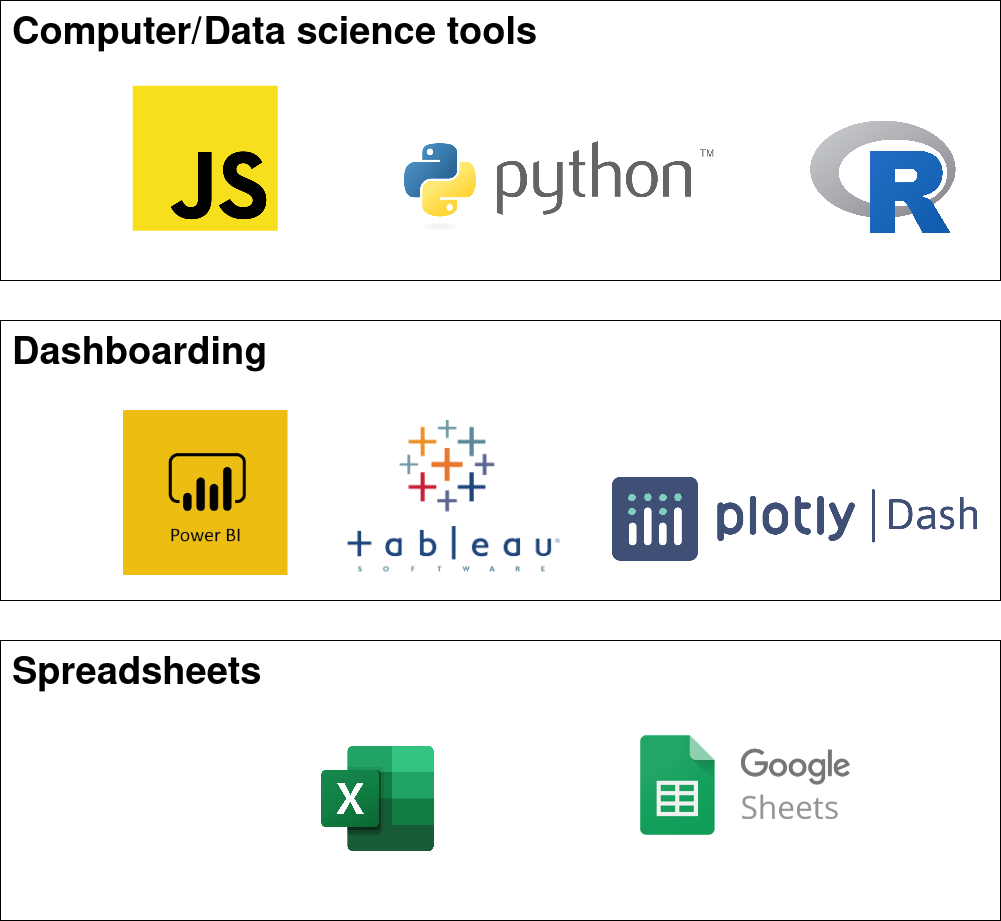
\includegraphics[width=0.7\textwidth]{img/viz/softwares.png}
\end{frame}



\section*{Best practices for Effective Data Visualization}

\begin{frame}{Best practice 1}

  \begin{block}{Consider your audience}
    \medskip
    \begin{itemize}
      \item Adapt your visualization to people
      \item Understand your audience’s area of expertise,
      \item[\textcolor{white}{x}] level of technical knowledge, and interests
    \end{itemize}
  \end{block}

  \bigskip

  \begin{columns}
    \begin{column}{.33\textwidth}
      
\includegraphics[width=\textwidth]{img/viz/BestPractice.png}
    \end{column}

    \begin{column}{.66\textwidth}
    \end{column}
  \end{columns}


\end{frame}

\begin{frame}{Best practice 2}
  
  \begin{block}{Clear the clutter}
    \medskip
    \begin{itemize}
      \item Avoid making unreadable, cluttered visualizations
      \item Ask yourself if what you’re including is relevant to the audience
      \item Remove unnecessary elements as much as you can
    \end{itemize}
  \end{block}

  \bigskip

  \begin{columns}
    \begin{column}{.33\textwidth}
      
\includegraphics[width=\textwidth]{img/viz/BestPractice.png}
    \end{column}

    \begin{column}{.66\textwidth}
    \end{column}
  \end{columns}
\end{frame}

\begin{frame}{Best practice 3}
  
  \begin{block}{Keep an eye on the fonts}
    \medskip
    \begin{itemize}
      \item One font with no more than three different sizes
      \item Respect the font hierarchy, keep headings larger than the body
      \item Use a bold typeface to highlight \textbf{key elements} and headings
    \end{itemize}
  \end{block}

  \bigskip

  \begin{columns}
    \begin{column}{.33\textwidth}
      
\includegraphics[width=\textwidth]{img/viz/BestPractice.png}
    \end{column}

    \begin{column}{.66\textwidth}
    \end{column}
  \end{columns}
\end{frame}


  
\begin{frame}{Best practice 4}
  
  \begin{block}{Use colors creatively}
    \medskip
    \begin{itemize}
      \item Color is one of the most eye-catching aspects of data visualization
      \item Choose a color scheme of your data visualization
      \item Use colors to hightlight groups, levels of importance, etc.
    \end{itemize}
  \end{block}

  \bigskip

  \begin{columns}
    \begin{column}{.33\textwidth}
      
\includegraphics[width=\textwidth]{img/viz/BestPractice.png}
    \end{column}

    \begin{column}{.66\textwidth}
    \end{column}
  \end{columns}
\end{frame}





\section*{Types of charts}

\begin{frame}{Overview}
  \centering
  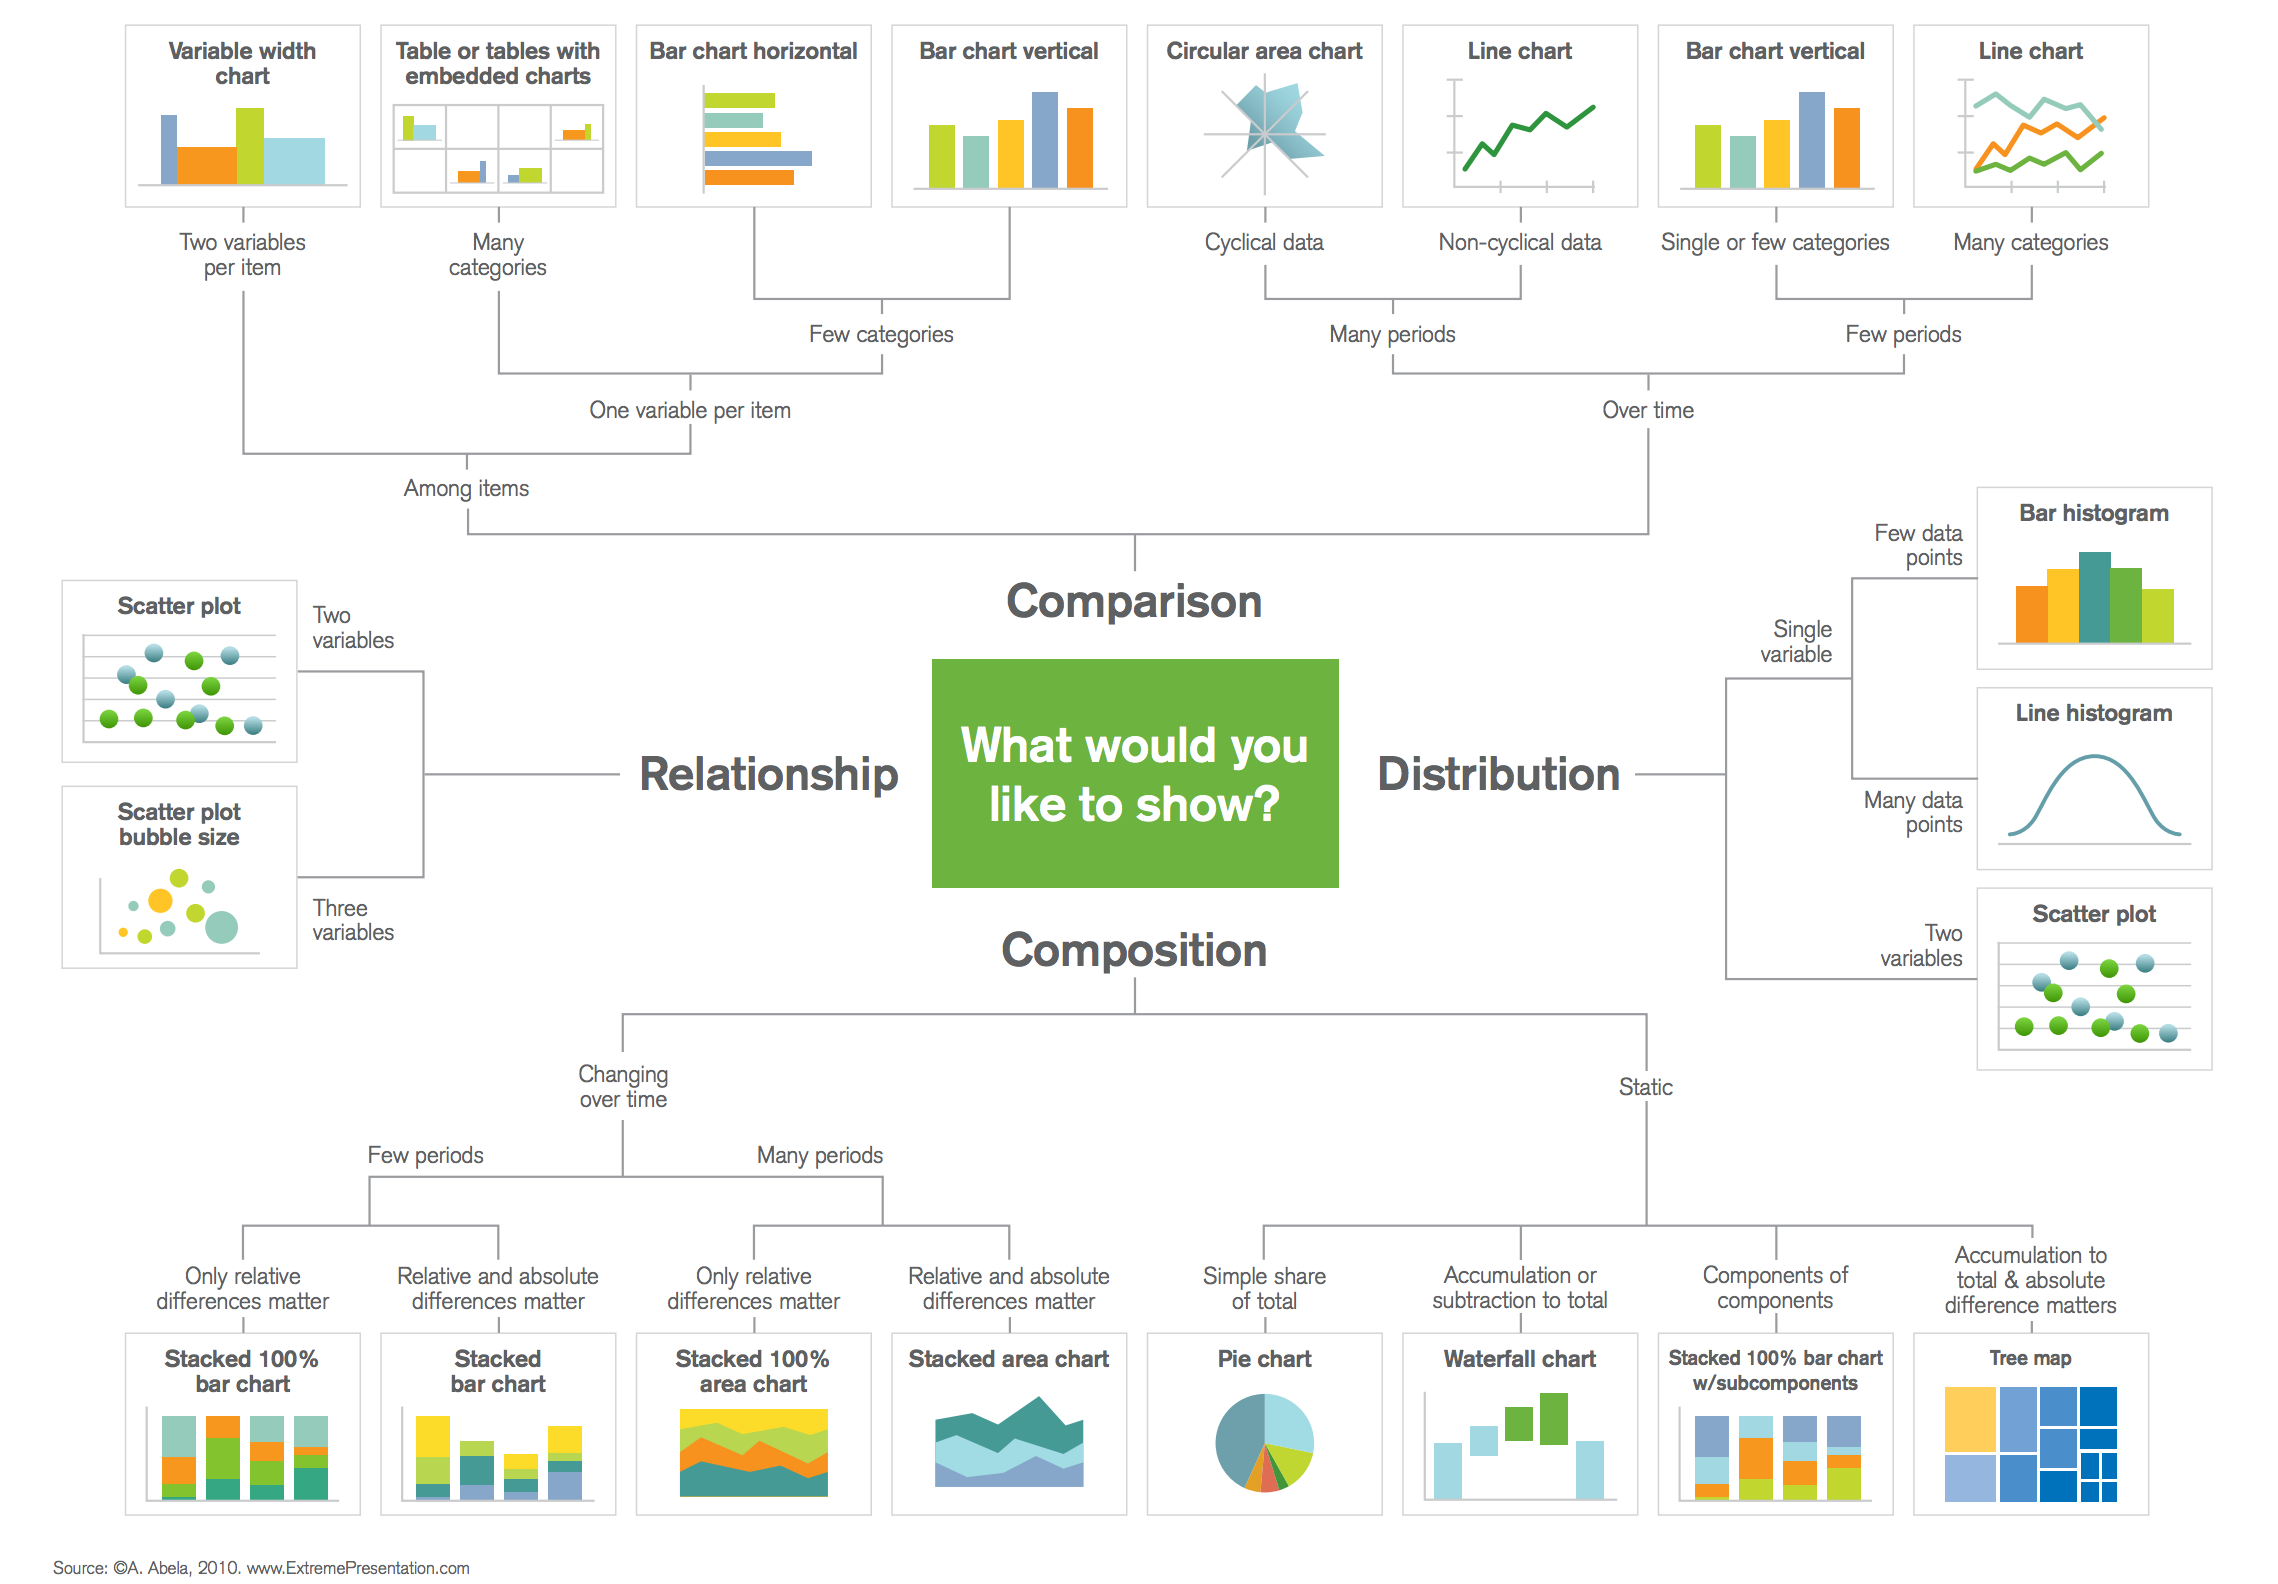
\includegraphics[width=\textwidth]{img/viz/chart-chooser-color}
\end{frame}

\begin{frame}{1D Bar chart}
  \centering
  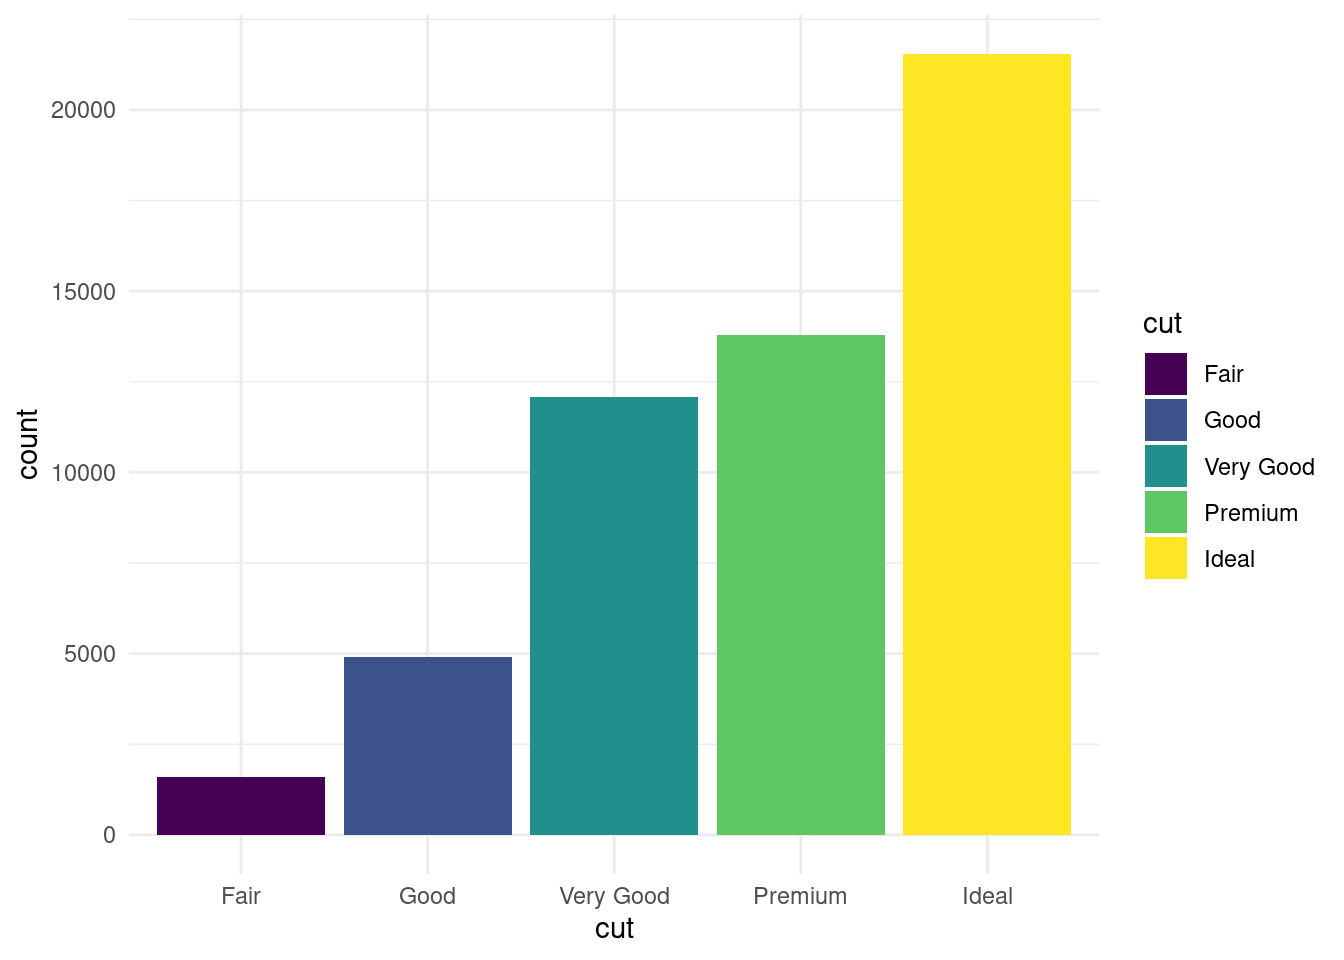
\includegraphics[width=.6\textwidth]{img/viz/barchart}
\end{frame}

\begin{frame}{1D Bar chart}
  \centering
  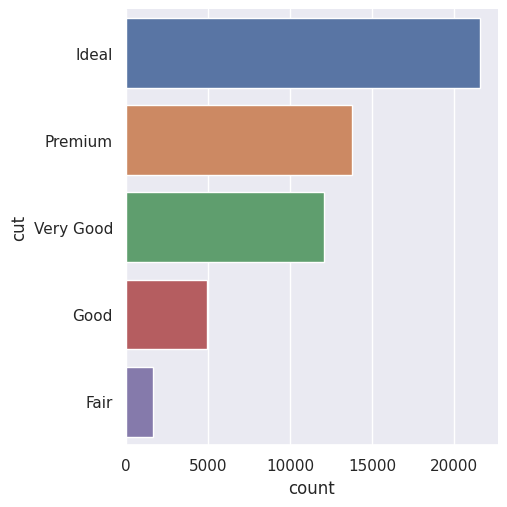
\includegraphics[width=.6\textwidth]{img/viz/catplot}
\end{frame}

\begin{frame}{1D Bar chart}
  \centering
  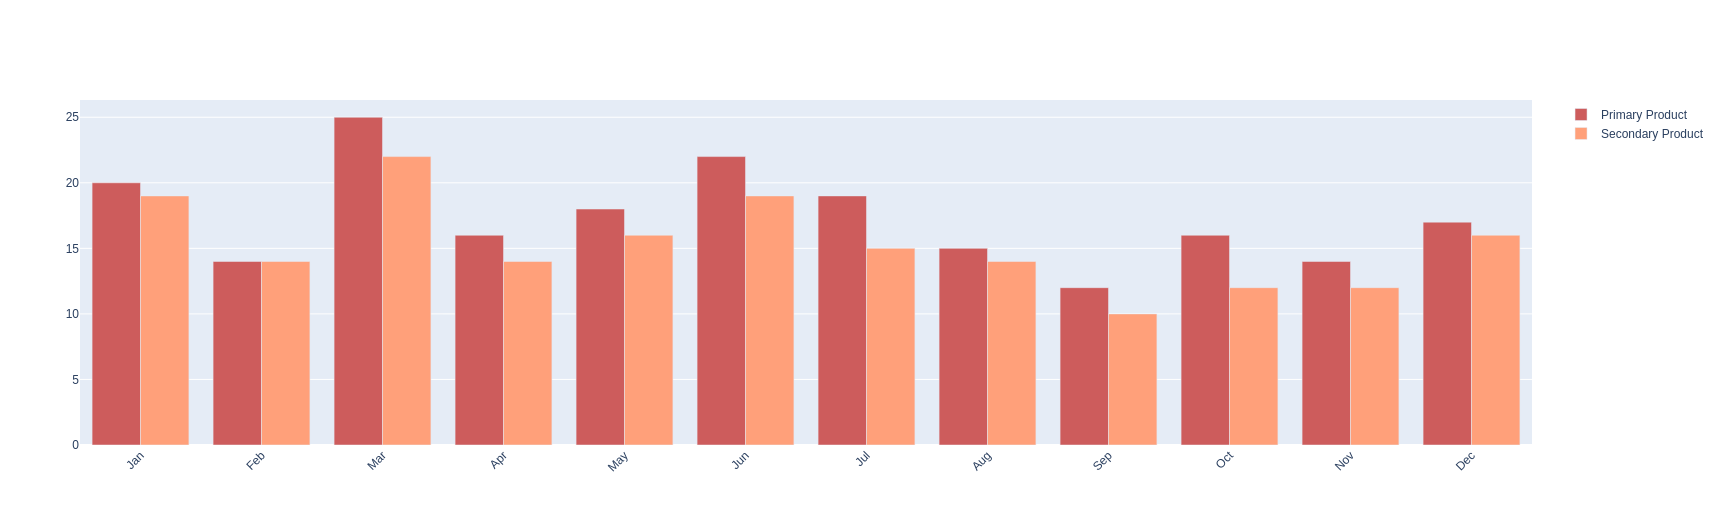
\includegraphics[width=\textwidth]{img/viz/barchart_grouped}
\end{frame}

\begin{frame}{1D Pie chart}
  \centering
  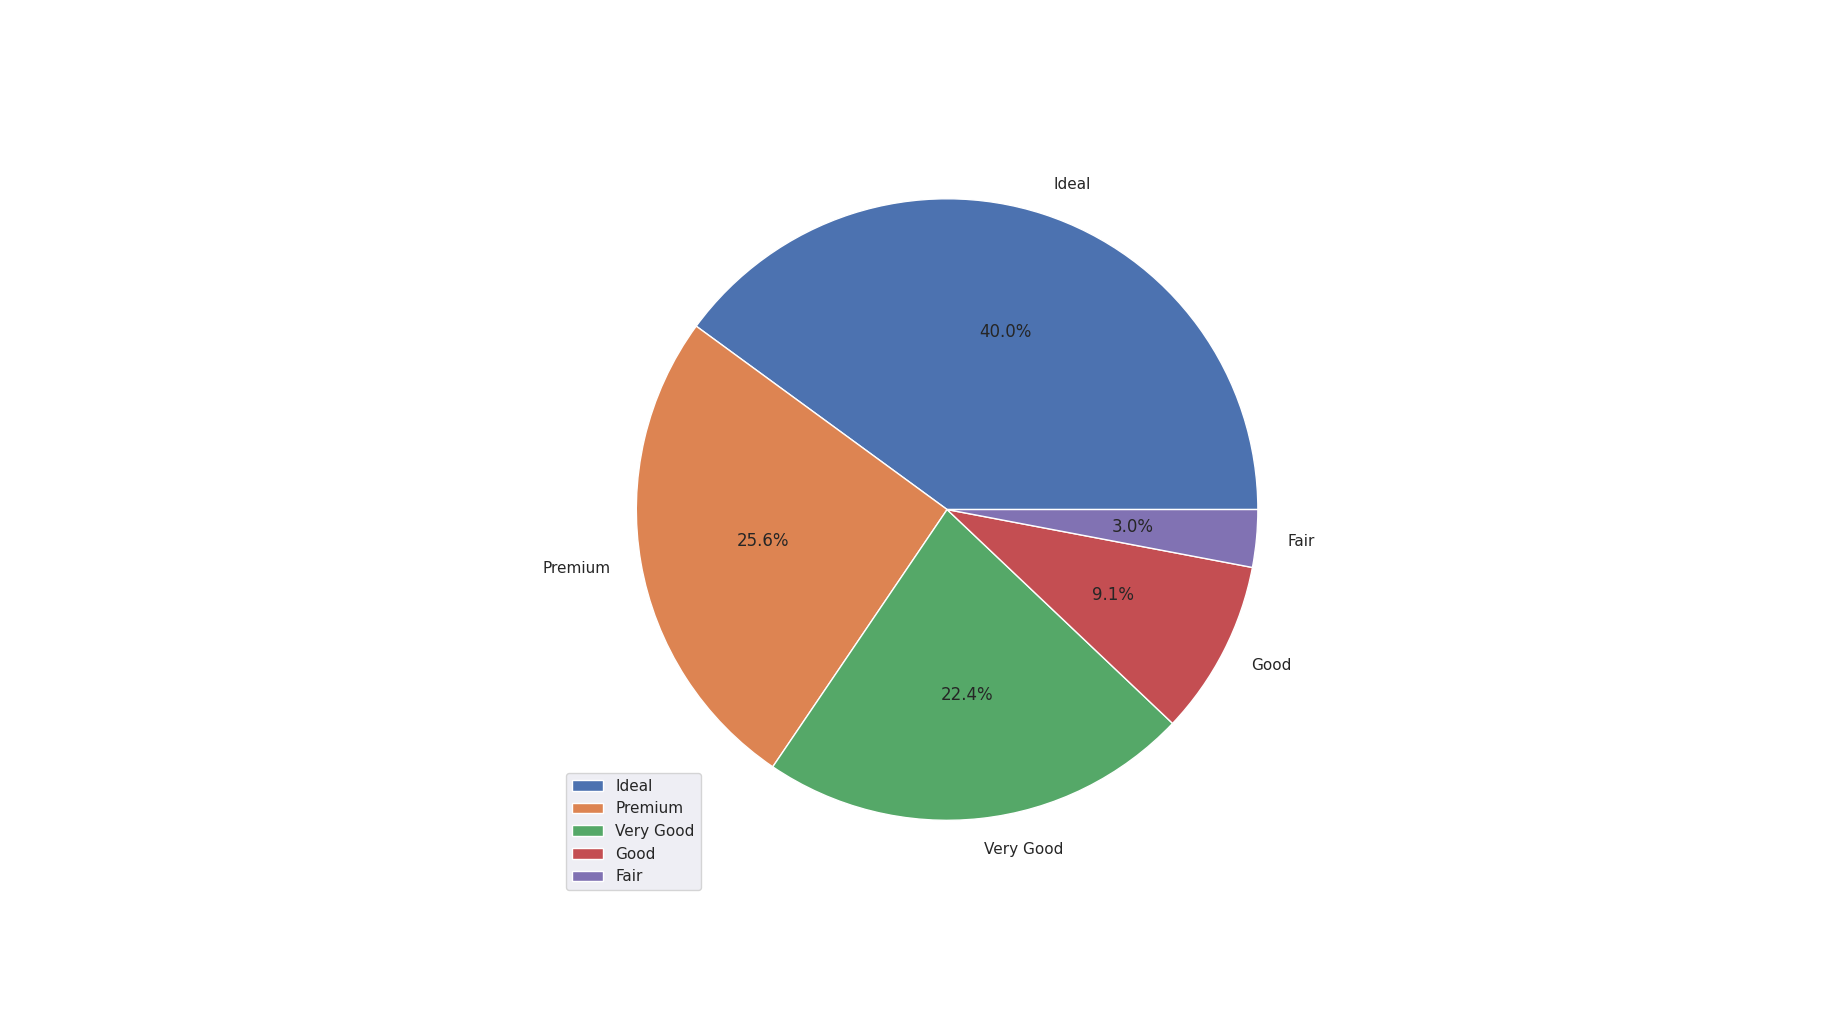
\includegraphics[width=\textwidth]{img/viz/pie}
\end{frame}

\begin{frame}{1D Pie and bar chart combined}
  \centering
  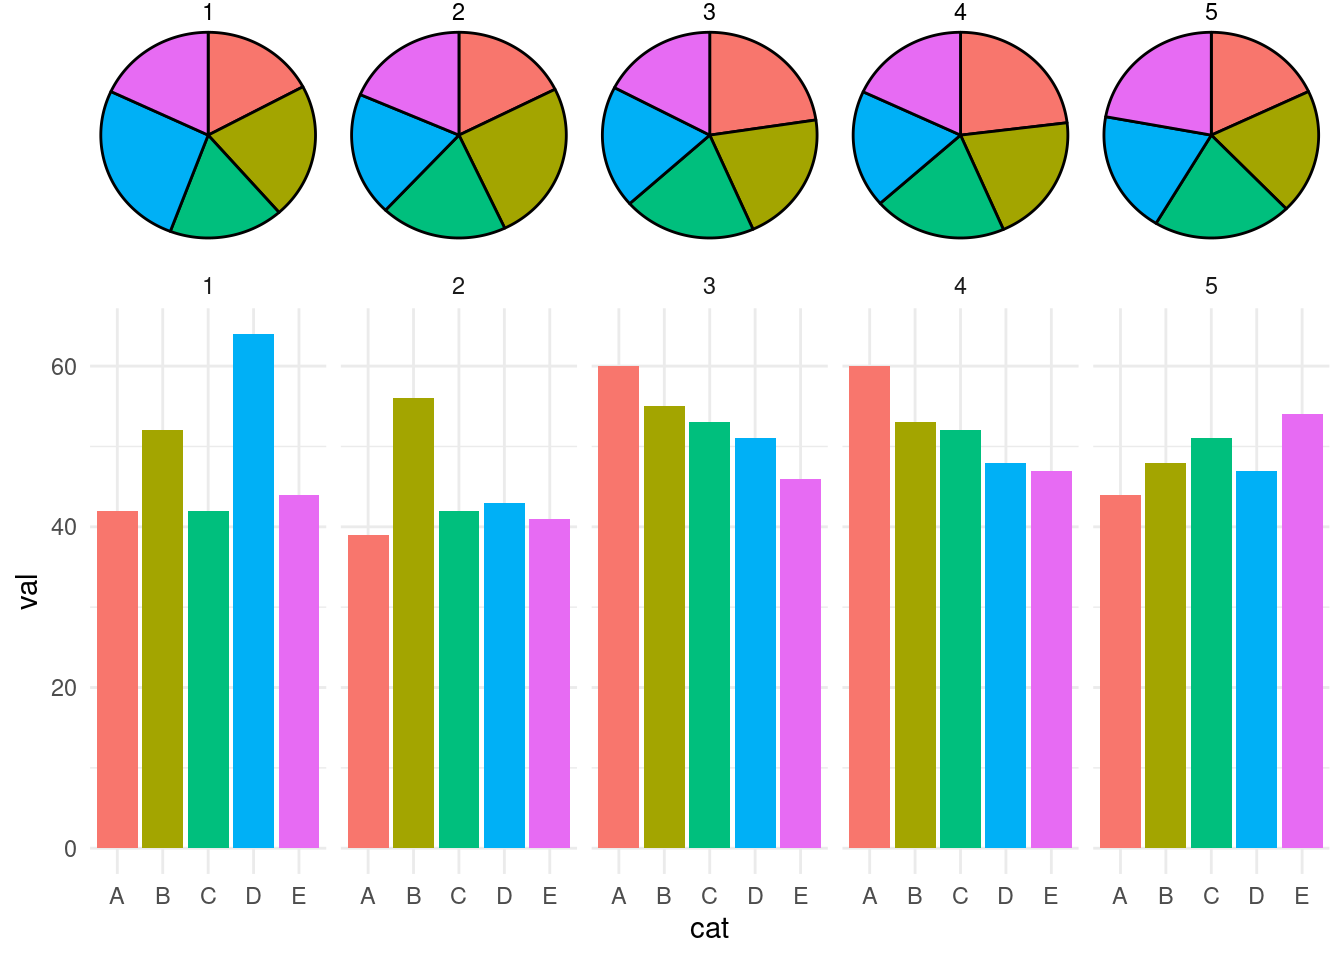
\includegraphics[width=.6\textwidth]{img/viz/bar_pie}
\end{frame}


\begin{frame}{1D Distribution: histogram}
  \centering
  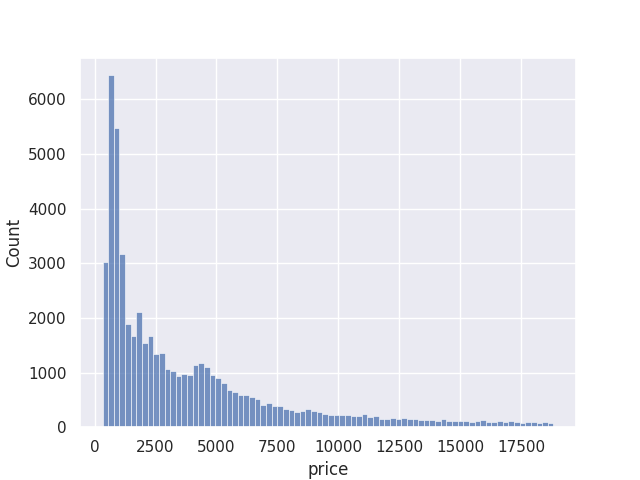
\includegraphics[width=.6\textwidth]{img/viz/histogram}
\end{frame}


\begin{frame}{1D Distribution: histogram}
  \centering
  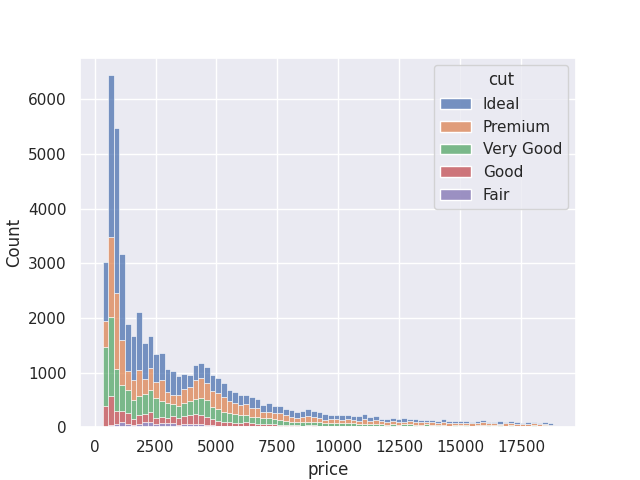
\includegraphics[width=.6\textwidth]{img/viz/hist_stacked}
\end{frame}


\begin{frame}{1D Distribution: density}
  \centering
  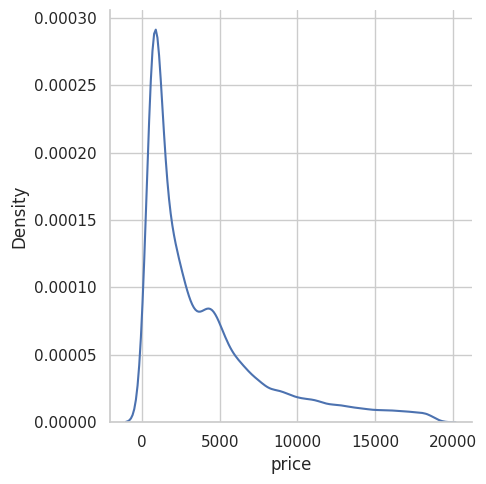
\includegraphics[width=.6\textwidth]{img/viz/kde}
\end{frame}


\begin{frame}{1D Distribution: density}
  \centering
  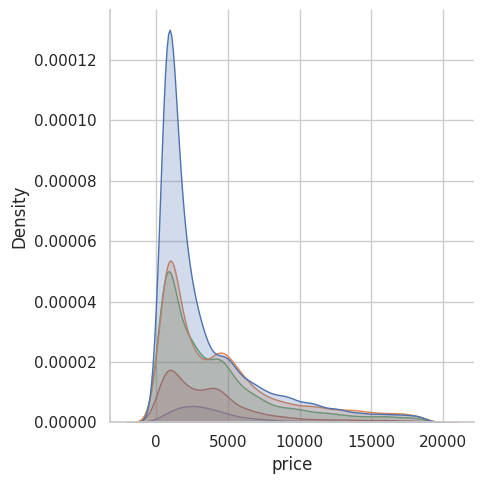
\includegraphics[width=.6\textwidth]{img/viz/kde_stacked}
\end{frame}

\begin{frame}{1D Distribution: box plot}
  \centering
  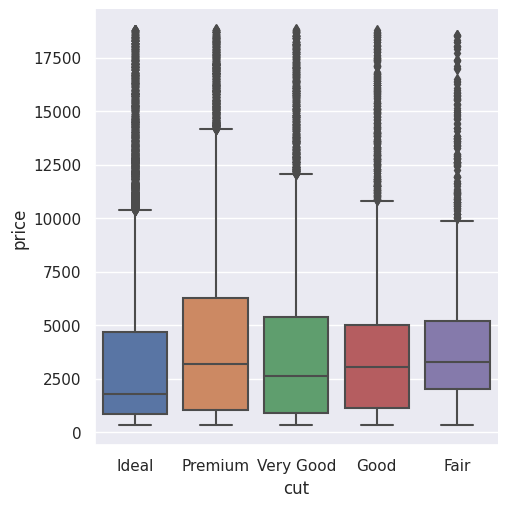
\includegraphics[width=.6\textwidth]{img/viz/box}
\end{frame}

\begin{frame}{1D Distribution: violin plot}
  \centering
  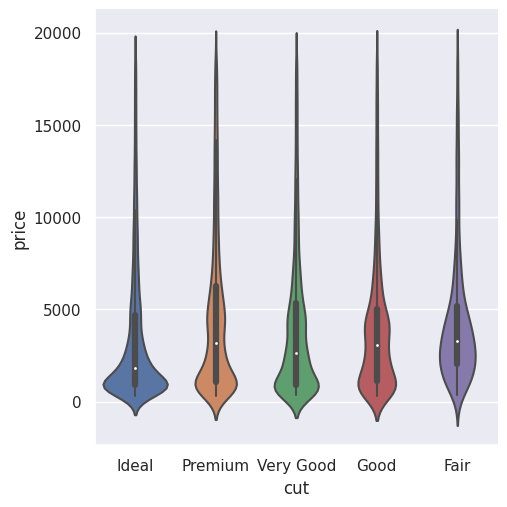
\includegraphics[width=.6\textwidth]{img/viz/violin}
\end{frame}


\begin{frame}{1D Time series}
\begin{block}{A sequence over the time}
  \centering
  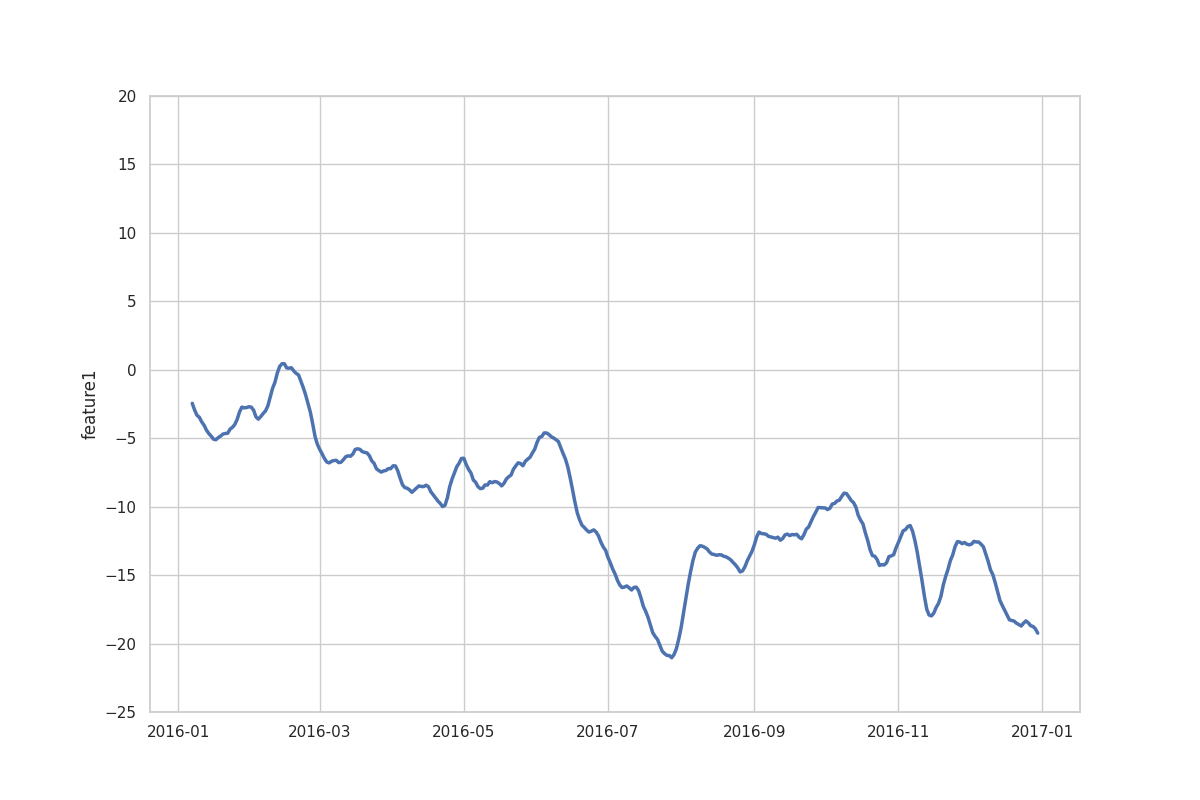
\includegraphics[width=.6\textwidth]{img/viz/line}
\end{block}
\end{frame}


\begin{frame}{1D Time series}
\begin{block}{A sequence over the time}
  \centering
  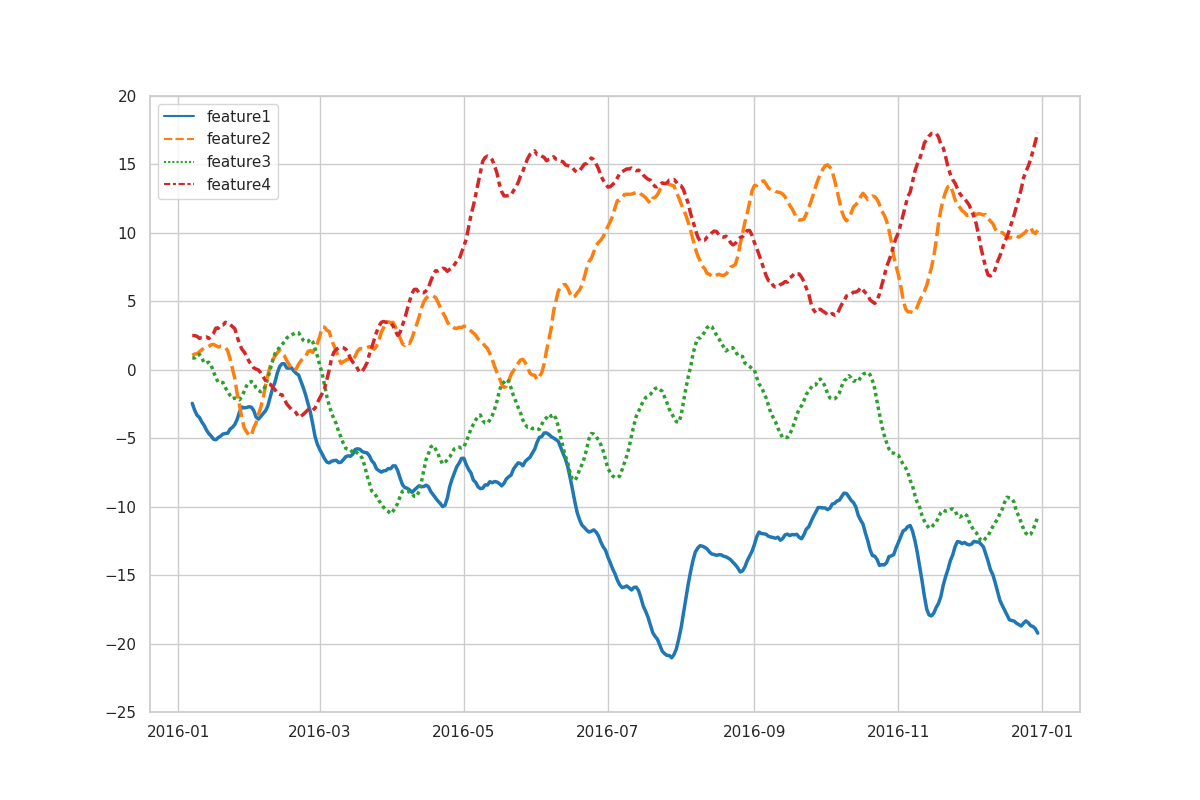
\includegraphics[width=.6\textwidth]{img/viz/line_cat}
\end{block}
\end{frame}


% 2D scatter, heatmap, pairplots, jointplot, kde

\begin{frame}{2D charts: scatter plot}
  \centering
  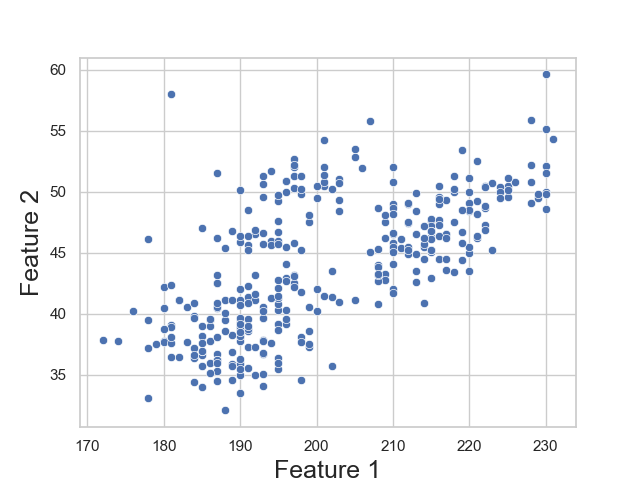
\includegraphics[width=.6\textwidth]{img/viz/scatter_2d_1}
\end{frame}

\begin{frame}{2D charts: scatter plot}
  \centering
  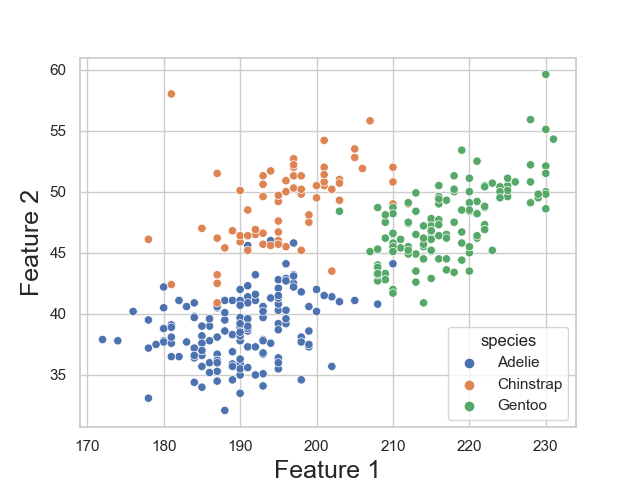
\includegraphics[width=.6\textwidth]{img/viz/scatter_2d_2}
\end{frame}

\begin{frame}{2D charts: scatter plot matrix}
  \centering
  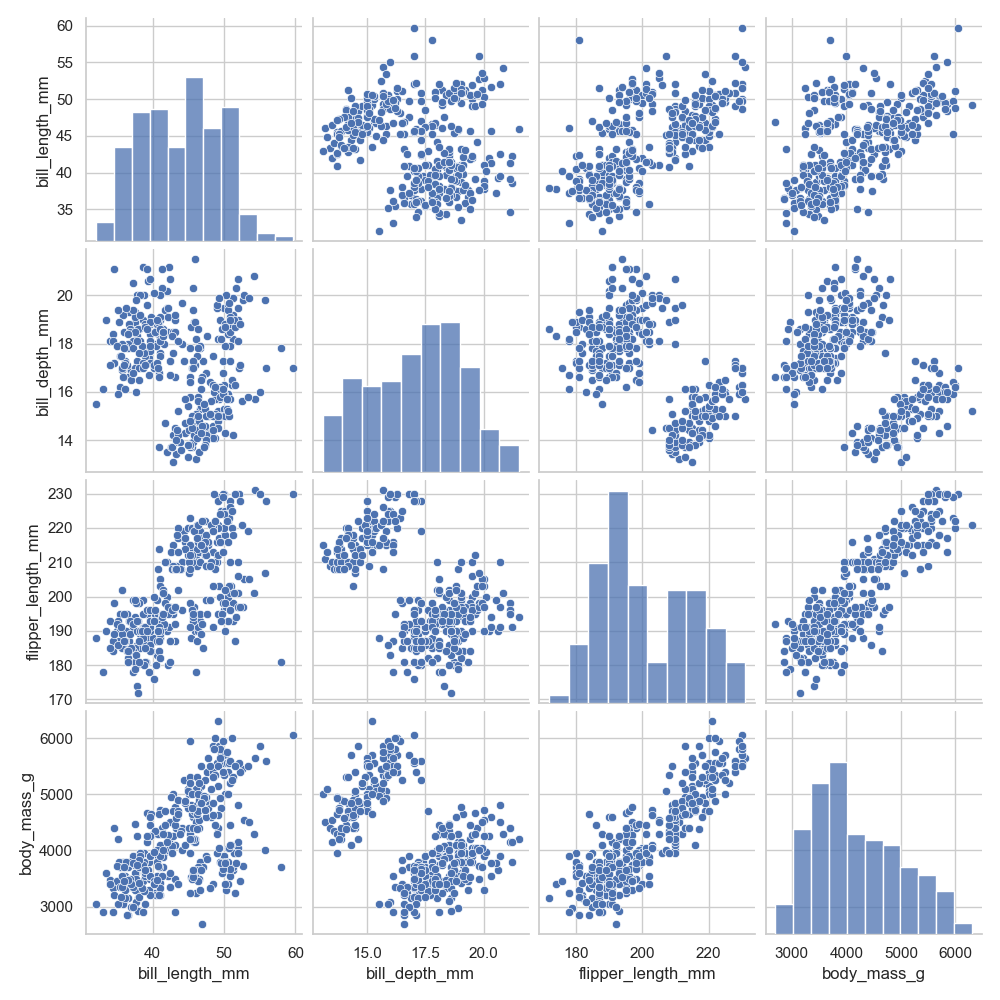
\includegraphics[width=.6\textwidth]{img/viz/scatterplot_matrix_1}
\end{frame}

  \begin{frame}{2D charts: scatter plot matrix}
    \centering
    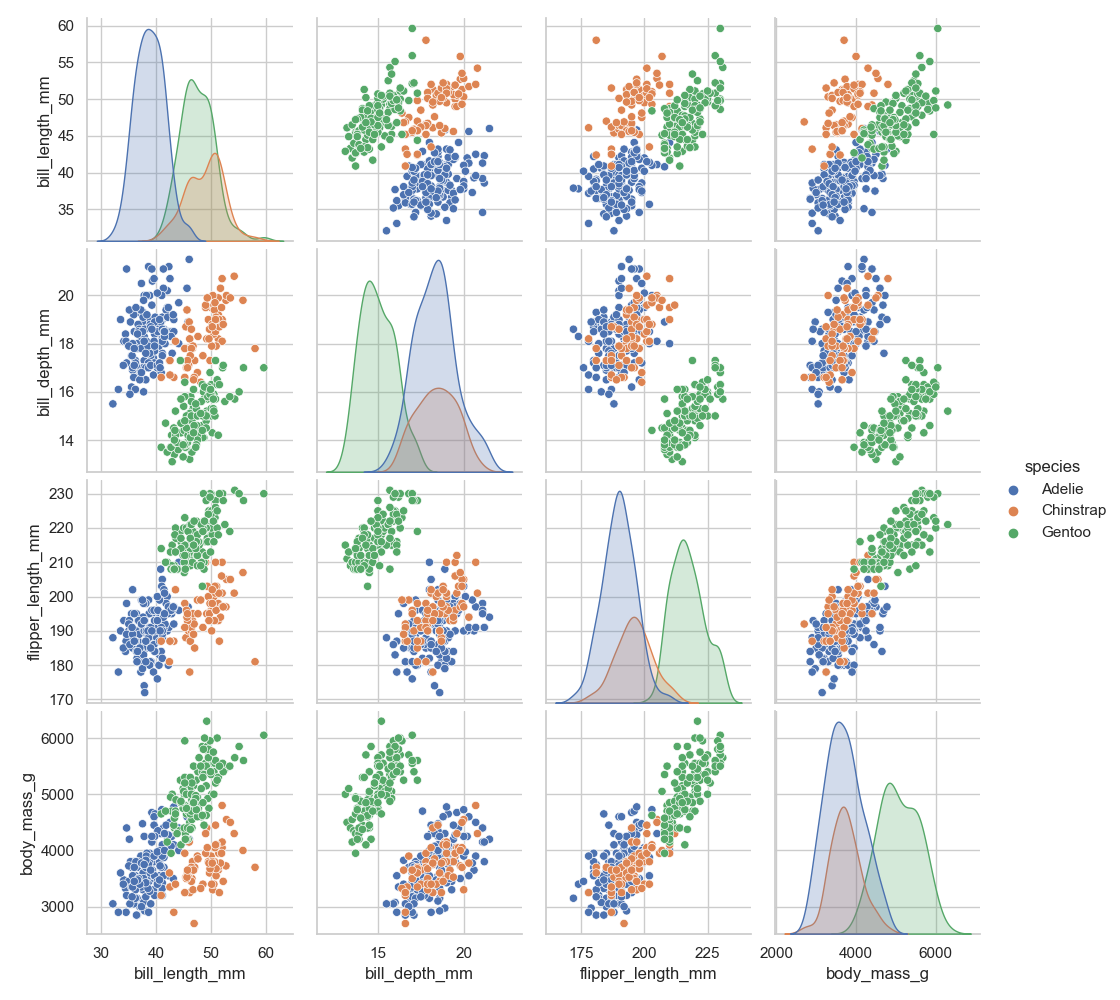
\includegraphics[width=.6\textwidth]{img/viz/scatterplot_matrix_2}
\end{frame}
      
\begin{frame}{2D charts: joint plot}
  \centering
  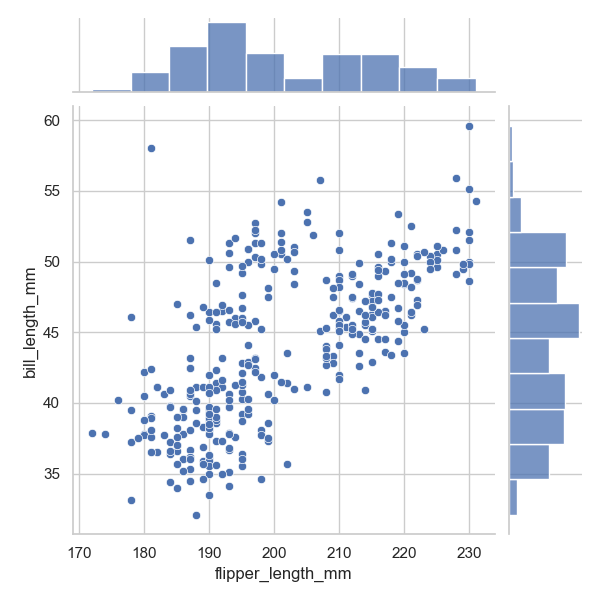
\includegraphics[width=.6\textwidth]{img/viz/jointplot_1}
\end{frame}

\begin{frame}{2D charts: joint plot}
  \centering
  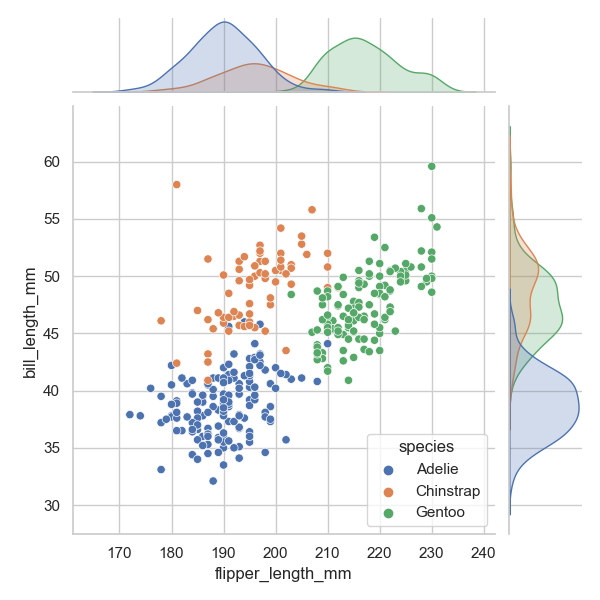
\includegraphics[width=.6\textwidth]{img/viz/jointplot_2}
\end{frame}




\begin{frame}{2D charts: heatmap}
\centering
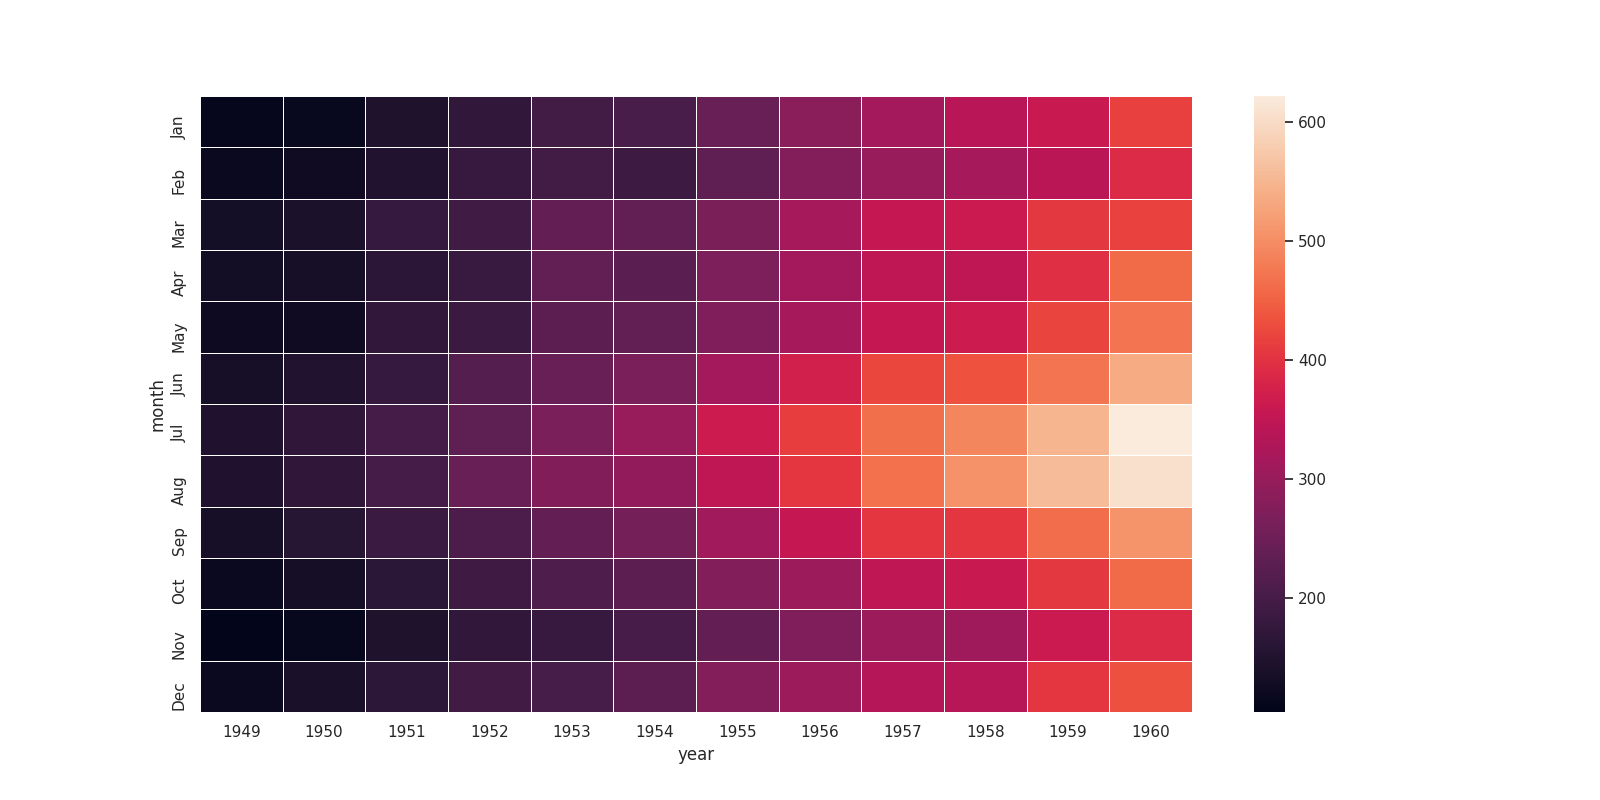
\includegraphics[width=1.2\textwidth]{img/viz/heatmap}
\end{frame}

\begin{frame}{2D charts: heatmap}
\centering
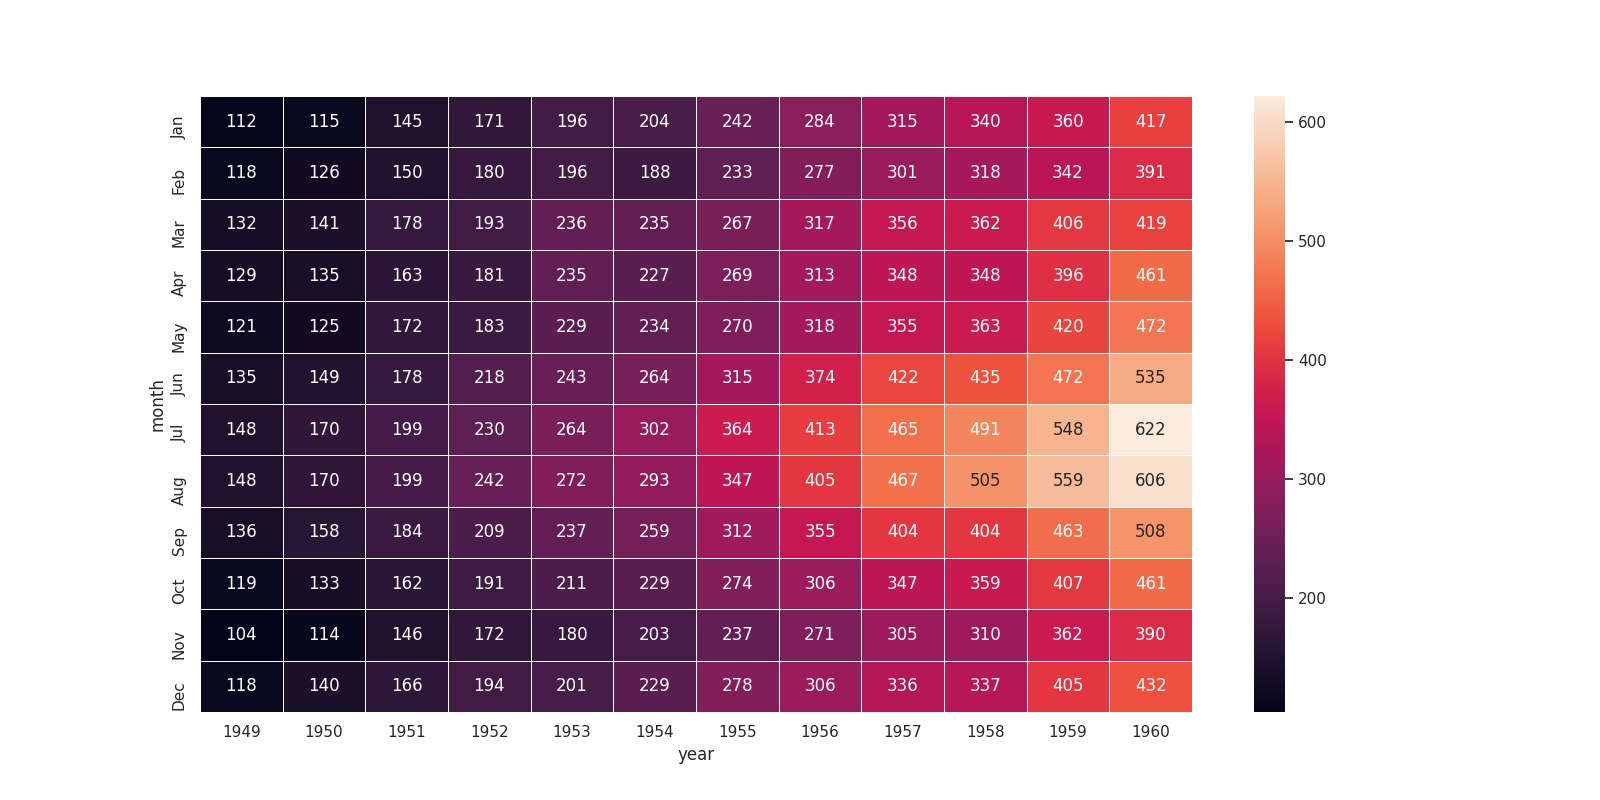
\includegraphics[width=1.2\textwidth]{img/viz/heatmap2}
\end{frame}




\begin{frame}{2D distribution}
  \centering
  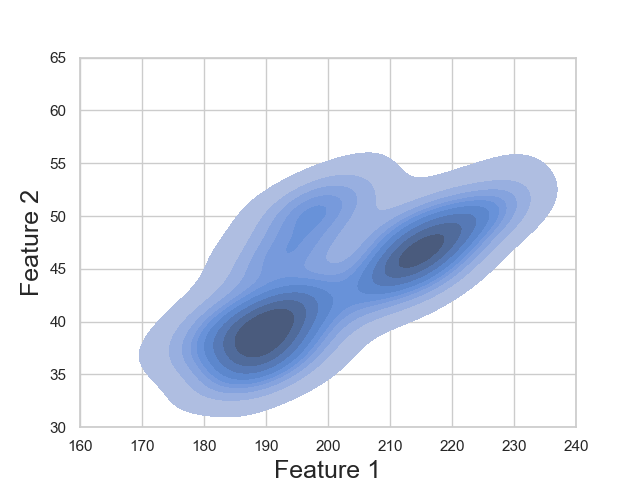
\includegraphics[width=.6\textwidth]{img/viz/kde2d_1}
\end{frame}


\begin{frame}{2D distribution}
  \centering
  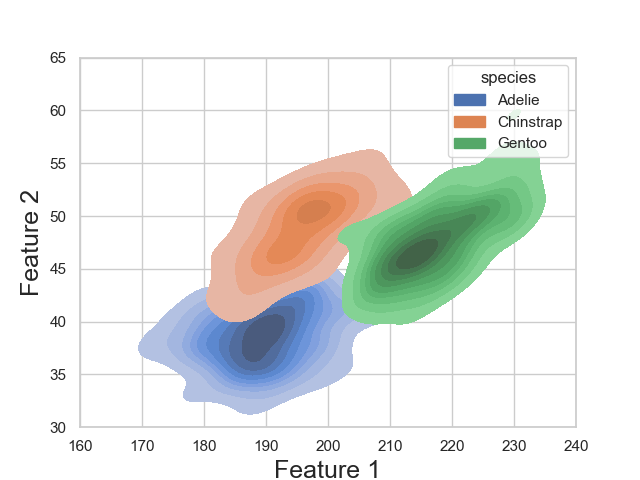
\includegraphics[width=.6\textwidth]{img/viz/kde2d_2}
\end{frame}

\begin{frame}{3D distribution}
  \centering
  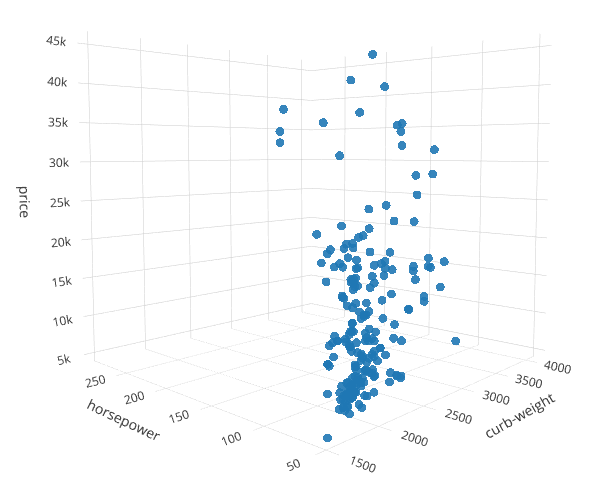
\includegraphics[width=.6\textwidth]{img/viz/scatter_3d}

  Source: \href{https://medium.com/@prasadostwal/multi-dimension-plots-in-python-from-2d-to-6d-9a2bf7b8cc74}{medium.com}
\end{frame}

% 4D to 6D scatter
\begin{frame}{High-dimensional: scatter plot}

  How to visualize points in a higher dimension than 3?

  \begin{block}{Key points}
    \begin{itemize}
      \item Add \textcolor{red}{colors} w.r.t. the values of an additional variable
      \item Add different \textcolor{red}{sizes} proportional to the values of an additional variable
      \item Add differnet \textcolor{red}{shapes} to the points
    \end{itemize}
  \end{block}

\end{frame}


\begin{frame}{High-dimensional: 4D scatter plot}
\begin{center}
  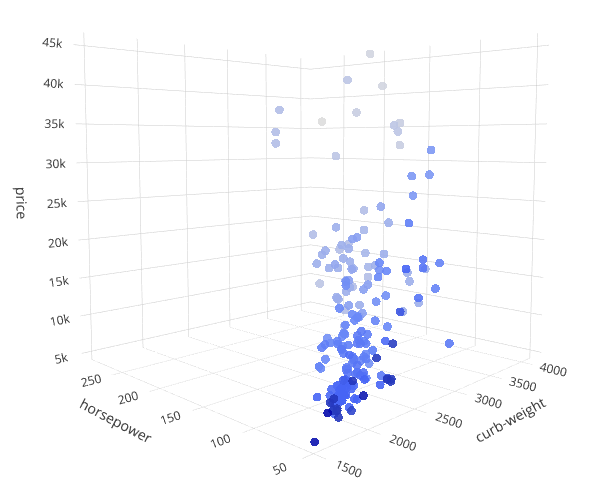
\includegraphics[width=.6\textwidth]{img/viz/scatter_4d}
  \begin{itemize}
    \item Add colors w.r.t. the values of an additional variable
  \end{itemize}
\end{center}

Source: \href{https://medium.com/@prasadostwal/multi-dimension-plots-in-python-from-2d-to-6d-9a2bf7b8cc74}{medium.com}
\end{frame}


\begin{frame}{High-dimensional: 5D scatter plot}
\begin{center}
  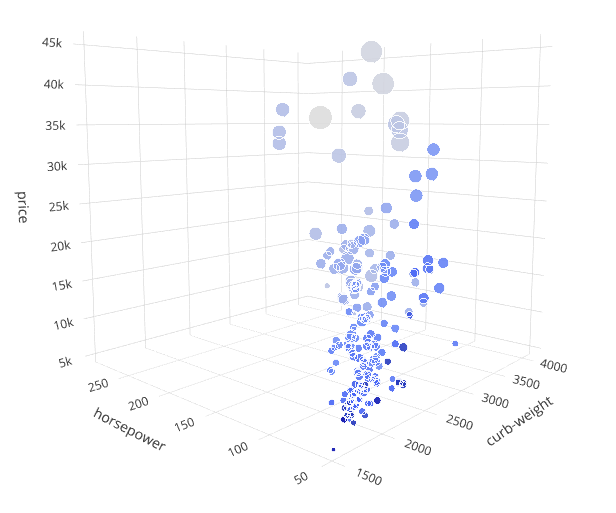
\includegraphics[width=.6\textwidth]{img/viz/scatter_5d}
  \begin{itemize}
    \item Add different sizes w.r.t. to the values of an additional variable
  \end{itemize}
\end{center}

Source: \href{https://medium.com/@prasadostwal/multi-dimension-plots-in-python-from-2d-to-6d-9a2bf7b8cc74}{medium.com}
\end{frame}


\begin{frame}{High-dimensional: 6D scatter plot}
\begin{center}
  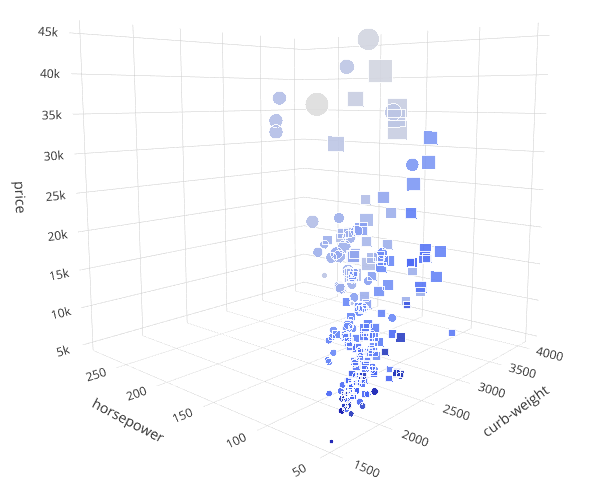
\includegraphics[width=.6\textwidth]{img/viz/scatter_6d}
  \begin{itemize}
    \item Add different shapes to the points
  \end{itemize}
\end{center}

Source: \href{https://medium.com/@prasadostwal/multi-dimension-plots-in-python-from-2d-to-6d-9a2bf7b8cc74}{medium.com}
\end{frame}


\begin{frame}{High-dimensional: radar plot}
  \centering
  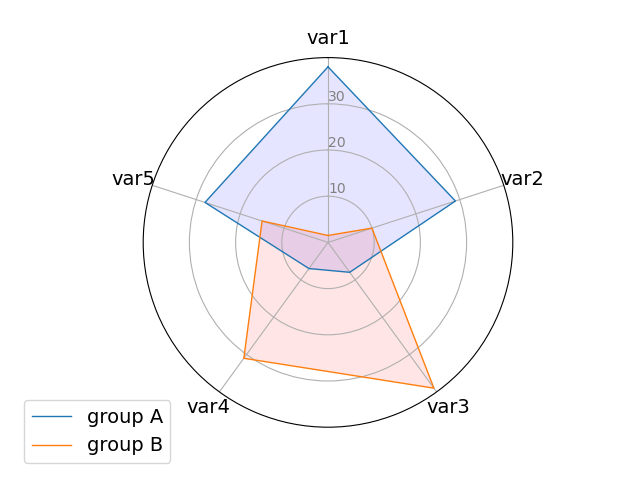
\includegraphics[width=\textwidth]{img/viz/radar}
\end{frame}


\begin{frame}{Maps}
  \centering
  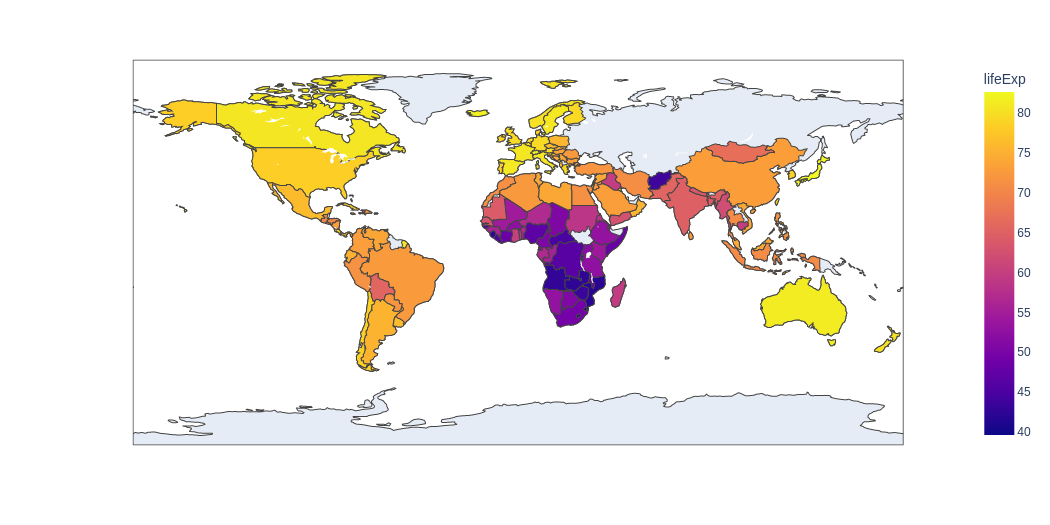
\includegraphics[width=.9\textwidth]{img/viz/map}
\end{frame}


\begin{frame}{Maps}
  \centering
  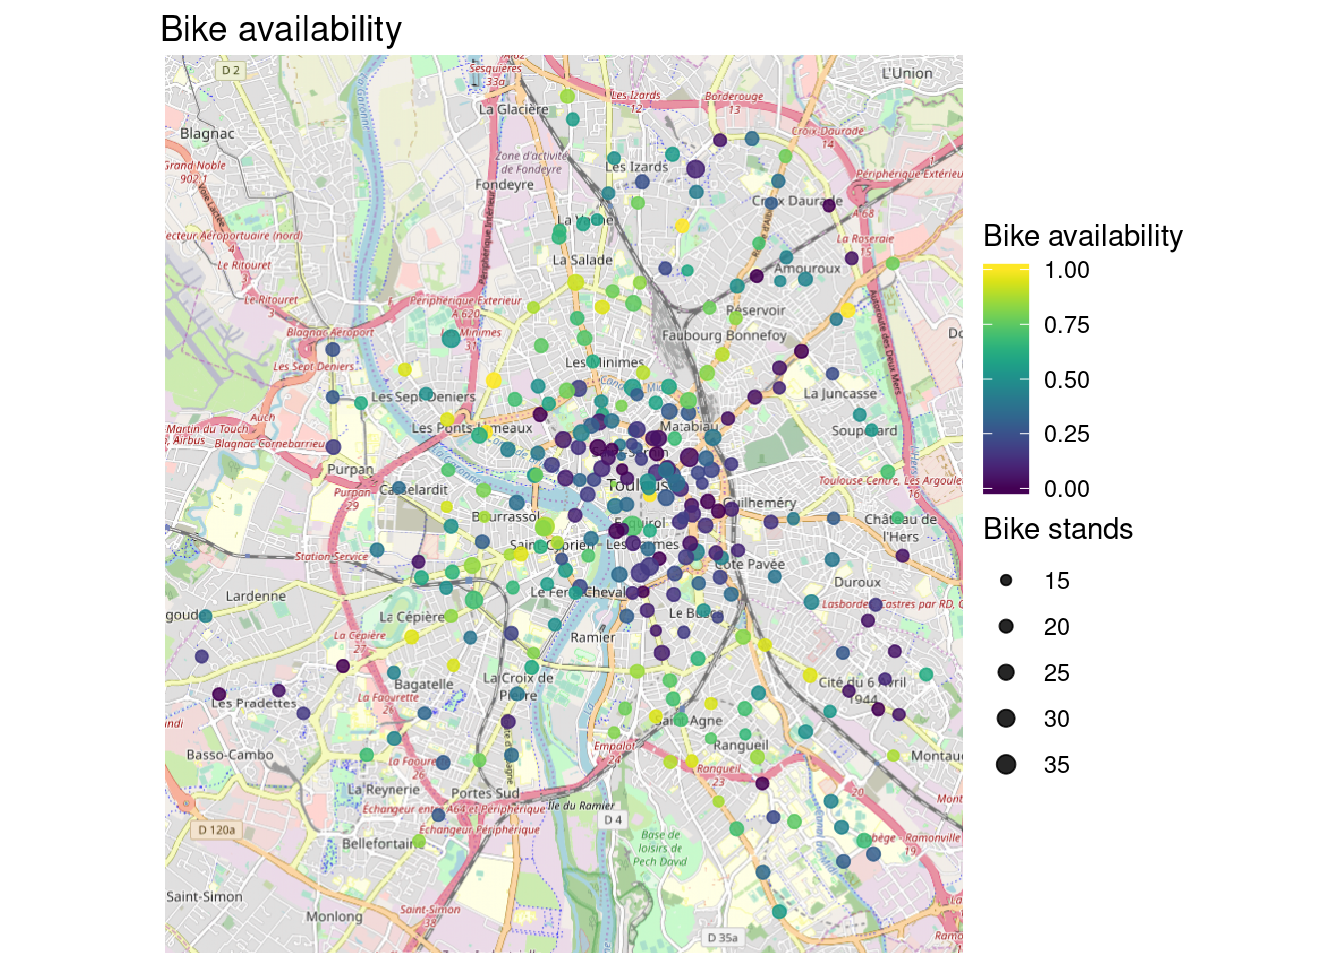
\includegraphics[width=.8\textwidth]{img/viz/map2}
\end{frame}

\begin{frame}{Networks}
  \centering
  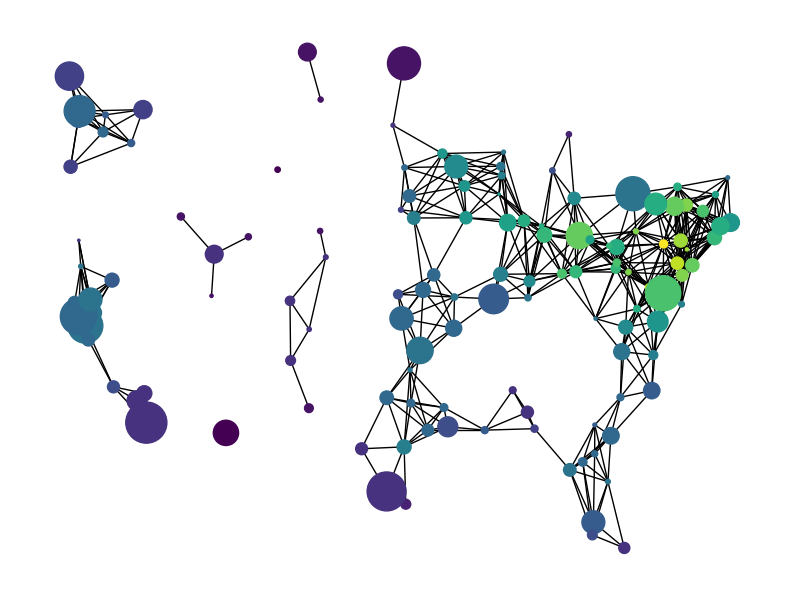
\includegraphics[width=.8\textwidth]{img/viz/network}
\end{frame}
